%%%%%%%%%%%%%%%%%%%% The_Report.tex %%%%%%%%%%%%%%%%%%%%%%%%%%%%%%%%%%%
%
% The AudioFiles Voice Chatting Report
%
% author: William McVicker, Tim Biggs, Chris Hoover
%
%%%%%%%%%%%%%%%% Springer %%%%%%%%%%%%%%%%%%%%%%%%%%%%%%%%%%


% RECOMMENDED %%%%%%%%%%%%%%%%%%%%%%%%%%%%%%%%%%%%%%%%%%%%%%%%%%%
\documentclass[letterpaper, 9 pt, balance, conference]{ieeeconf} 

\usepackage{float}
\usepackage{amsmath}        % need for equations
\usepackage{mathptmx}       % selects Times Roman as basic font
\usepackage{helvet}         % selects Helvetica as sans-serif font
\usepackage{courier}        % selects Courier as typewriter font
%
\usepackage{makeidx}         % allows index generation
\usepackage{graphicx}        % standard LaTeX graphics tool
\usepackage{subfig}
                             % when including figure files
\usepackage{multicol}        % used for the two-column index
\usepackage{balance}
% see the list of further useful packages
% in the Reference Guide

\makeindex             % used for the subject index
                       % please use the style svind.ist with
                       % your makeindex program

\newcommand{\thickhline}{\noalign{\hrule height 1.0pt}}
\newcommand{\tab}{$\hspace{6pt}$}
\newcommand{\mathbi}[1]{\textbf{\em #1}}
%%%%%%%%%%%%%%%%%%%%%%%%%%%%%%%%%%%%%%%%%%%%%%%%%%%%%%%%%%%%%%%%%%%%%%%%%%%%%%%%%%%%%%%%%

\begin{document}

\bibliographystyle{IEEEtran}

\title{Audio Data Transmission using DCCP Transport Protocol}

\author{\authorblockN{Chris Hoover\authorrefmark{1}, Tim Biggs\authorrefmark{1}, William McVicker\authorrefmark{1}}$\vspace{3pt}$
\authorblockA{\authorrefmark{1}California Polytechnic State University\\
   San Luis Obispo, CA 93407 USA\\%
   Email: chhoover@, tebiggs@, wmcvicke@calpoly.edu}%
}

\maketitle
\IEEEpeerreviewmaketitle

\begin{abstract}
\boldmath 
This paper aims to build a framework that utilizes the Data Congestion Control Protocol (DCCP) in order to experimentally test its congestion control system.  DCCP is a hybrid between TCP and UDP in that it offers congestion control across an unreliable transmission protocol along with a connection-oriented setup and teardown design. Applications that do not require a reliable connection, but desire to trasmit data at high rates are the ideal users of DCCP. Applications include audio streaming, video streaming, and video games. In this paper we propose the design of an audio chatting application that has a framework capable of swapping out different transport layer protocols in order to test the performance of DCCP. The three protocols used for out application are: DCCP, TCP, and UDP. By abstracting out the transport layer at the application level, we can easily compare and contrast the differences in jitter and packet loss between the three different transport layer protocols in an audio streaming/chatting environment. We found that UDP was the least affected by network congestion.  DCCP was not significantly affected between high link utilization and full link utilization with regards to our chosen metrics. Between DCCP and TCP, we found DCCP having a higher average packet loss percentage than the other two protocols.  For jitter, DCCP had a steeper change in jitter over time where TCP had a more graduale increase in jitter over time. Overall, we found the congestion contol system implemented in DCCP to behave similar to how TCP behaves with slightly more packet loss for DCCP.

\end{abstract}

\section{Introduction}
\label{sec:intro}

Data Congestion Control Protocol (DCCP) is a transport layer protocol that implements congestion control without the reliability of TCP~\cite{kohler06}. It contains the benefits of unreliability provided by UDP along with the congestion control system found in TCP. In essence, DCCP is a hybrid between UDP and TCP. The need for a protocol such as DCCP arose due to the need for congestion control for applications for which TCP is not an appropriate solution. Because UDP ignores packet performance when sending over the network it will simply send packets as fast as possible, generally resulting in a higher amount of lost data. By contrast, TCP will keep data integrity, but because packets may be retransmitted multiple times it is not very applicable for time-sensitive applications that rely on not being blocked when a packet gets dropped.

DCCP is currently at the proposed standard RFC status (4340-4342). It is available for use through the linux socket library~\cite{dccp_website}. Its main goal was "to give streaming UDP applications little reason not to switch to DCCP"~\cite{dccp_wg} by requiring as little overhead as possible with full functionality. The design of DCCP was geared mostly toward media streaming applications which include audio, video, and gaming software where responsiveness is traded for a steadier, less bursty network connection.

The main goal of this paper is to evaluate DCCP's congestion control performance by implementing a voice chatting application with DCCP as the underlying audio transmission protocol.  The voice chatting framework was designed to allow the user to choose between DCCP, UDP, and TCP as the transport layer protocol for transmitting audio packets between clients. This is done by building a framework that abstracts out the transport layer protocol at the application layer. With this framework, we can also observe differences in speed, jitter, and packet loss.

\section{Background}
\label{sec:backg}

The most popular transport layer protocols in use today are TCP and UDP. Though other protocols do exist, these are the most commonly used ones, particularly throughout industry as a whole. TCP is known mainly for it reliability and its congestion control system while UDP is known mainly for its best effort approach that favors timeliness over reliability. The increase in media streaming over the past decade has greatly illustrated the need for efficiency of sending data without the reliability. UDP gives us the basic tool to do this. By streaming over an unreliable protocol and avoiding retransmissions, it is faster and easier for people to process. We can handle skips from time to time, but it's harder for us to handle consuming such media out of order. However, when transmitting data that requires file integrity, such as an archived tarball, a reliable protocol must be used. TCP was designed for this very reason and is widely used as the standard reliable transport layer protocol.

Though TCP and UDP address many of the connections needs for various applications, there has been a growing need for an additional protocol. Let's consider what happens when we send data over a congested network. Because TCP has an aggressive back-off when it detects congestion and because it will attempt to retransmit packets (even over a congested network), it is not a suitable candidate for applications attempting to do media streaming. By contrast, UDP will send packets as fast as possible regardless of whether the network is congested or not, which could result in much more irregularity (and higher drops) in the arrival of packets for the receiver. Although these protocols have their ways of dealing with network congestion, they are not always the appropriate solution depending on typical network conditions and needs of the application.

DCCP was designed for this very purpose: to support congestion control where a less reliable connection is sufficient. The authors of DCCP created the protocol with the primary goal of supporting congestion control without reliability, and in doing so discovered some of the complexities of TCP and how it is able to work so well.

\section{Architecture}
\label{sec:architec}

\begin{figure}[h]
   \centering
      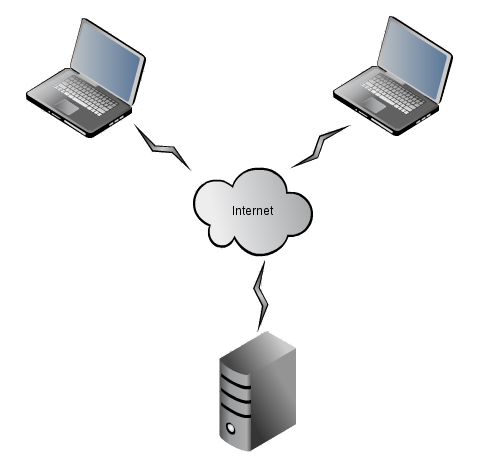
\includegraphics[width=0.4\textwidth]{pics/setup}
   \caption{High-level diagram of how the voice chatting application is setup.}
\label{fig:setup}
\end{figure}

We designed our voice chatting application to work with many different clients at once. Each client communicates with a central server to retrieve information about calling other clients and to keep track of who it can actually call. The server maintains a database used to authenticate each user upon starting the application. After logging into the system, the server is used as an intermediary for the clients to retrieve current information about the user's friends' statuses, hostname, and port number. This information can be used to request a chatting session with another client that is logged onto the server.  Fig.~\ref{fig:setup} shows a high-level network topology representation of what a set of clients logged into this chatting application would look like.  The server and client subsystems are described in the following sections.


\section{Server Overview}

In order to negotiate the connection setup between two or more clients, we decided to
design and implement a server application. The server 
manages the clients' connection statuses, similar to an instant messaging
server.
It provides a method for clients to sign on or off, a way to check friends' online
statuses, and a method to request a friend's ip address and port.

\subsection{Server Design Decisions}

We had to make a number of design decisions for the server, which are described here.

We'll start with the choice of implementation language. Because the server is a
separate entity from the chat client, we had some extra freedom for language and
design choice. The primary requirement for the server was that it must be able
to connect and communicate with each client. After some consideration, we
implemented the server in Python for two main reasons. First, Python
has a number of modules, including a socket-based asynchronous server, available
to aid with development. Second, Python's general syntax and ease of use makes
it a great tool for creating mock-ups or relatively small, short-term projects.
Of course, it works well for larger projects too. Python made coding much
cleaner and more maintainable for the goals of our project.

We wanted the server to perform some of the same capabilities that a
watered-down chat server (such as one used for Skype) might have or use. To that
end, we needed it to have login functionality and user tracking. We determined
that the server had to perform the following tasks at minimum.

\begin{enumerate}
  \item Provide a way for a user to register that he or she is online.
  \item Provide a way for users to talk to each other.
  \item Maintain a list of users each client is permitted to contact.
  \item Provide information updates to each user about their friends' online statuses.
\end{enumerate}

The first task is essential because it represents the core reason for adding a
server element: to keep track of users. By giving users a way to register that
they are connected (and conversely, allow them to disconnect as needed), the
server could keep track of users as they log in or log out, allowing it to
perform additional functionality. This is also required for task 4 and is the
basis of the notification system on the client side.

The second task is important because users shouldn't be expected to know the IP
address or port number of the computers their friends are on. The client needs a
way of obtaining this information from the server, and thus being able to chat
with others. It is important that this information be maintained by the server
so that users have more freedom when using our system. When testing, it also
provided the benefit of not needing to manually enter in a new IP address/port
number combination every time we want to initiate a chat session. The main
drawback for this feature is that a client must request for this information
every time he or she wants to start a chatting session with one of his or her
friends.

Strictly speaking, only points 1 and 2 above are actually needed for a
minimalistic server to function. The server keeps track of who is online, and
tells clients where they can contact other clients who are online. However, we
wanted our server to emulate some additional features seen in commercial media
streaming applications. This leads to our third task: maintaining a friends list
for each client.
The server keeps a list of who is friends with whom, thereby limiting clients from being able to randomly call or spam other users who might be online.

The final task is fairly closely related to task 3. In order to cache friend
information on the client side (so the client won't make chat requests for
offline users), the server should be capable of periodically sending updates to
each connected client. These updates notify the client of which of his friends
he is able to call at any given time.

Our final core design choice relates to storage of user information. As it is
standard in industry, we decided the server should store information in a
database file that is easily accessible without any parsing or configurations.
In this database, the server would keep track of user and friend list
information, as well as any other necessary information needed, i.e. IP
addresses and port numbers. Although it isn't very much information to keep
track of, it still gives a relatively simple solution to keeping track of users
without the overhead of having to store information manually (such as in a text
file).
 
\subsection{Server Implementation}
Now that we've covered the key design decisions of the server, we will describe how the server
was implemented. A generalized state diagram is shown in Fig.~\ref{fig:server_diag}.

\begin{figure*}[!t]
   \centering
      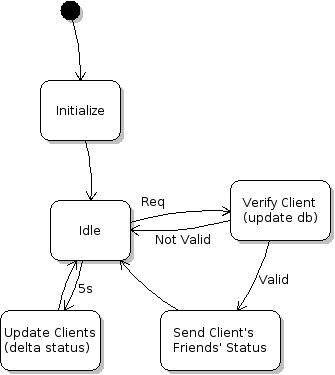
\includegraphics[width=0.8\textwidth]{pics/Server_StateDiagram}
   \caption{Server State Diagram demonstrating the general flow of the central server.}
\label{fig:server_diag}
\end{figure*}


Python has a number of different modules available for applications to communicate
through using network sockets. Our first consideration was the SocketServer module. This 
library
provides an interface which can block receive requests, and then execute a request
handler via a callback. Unfortunately, this module has one major flaw: it can only handle
one user request at a time. Because the server needed to handle multiple connected users
asynchronously, we settled on using the asyncore module. This module has essentially
the same functionality as SocketServer, but with asynchronous I/O and support for multiple clients. With this module, each
new incoming connection request from a client executes a request handler in its own seperate thread, allowing 
multiple clients to connect and remain logged in at the same time.

To allow clients to log on, request information, and receive updates, it made
sense for the server to use a reliable connection-oriented protocol. Thus, TCP was the 
natural
choice for client to server communication. When a client connects to the server, the server spawns a new thread to maintain
the connection to the client. If the client makes any requests, the response packets will 
be sent
directly to the child thread connected to that client instead of the main server loop. Each child thread has its own
instance of a request handler that controls the logic for reading, interpreting, and replying
to each client request. If a client closes its connection, the thread closes as well and is
removed from the loop. 

To log in, a client establishes a connection to the server (in our tests
the client would accept the IP address of the server as an input parameter) and sends it
a packet with two 20 byte strings: a username and a password, padded as necessary with
null bytes. The server then accepts the packet, verifies the username and password, and
replies back to the client with either a success or failure packet depending on the
validity of the credentials. The password is sent over the network as plaintext (normally
it would be encapsulated in an SSL connection) and the server, upon reception, hashes
the password with a salt using an SHA-512 function and compares the result to the stored hash value 
in the database. If the hashes match, the user is granted login privileges. This
security isn't hack-proof, but it at least models a standard login procedure.  Additional
security concerns are left for future work.

Once a client successfully logs in, the server replies back with a friend list packet.
This packet contains a list of usernames and IDs for all the client's current
friends.
This packet does not contain any online statuses, and in the event of an overflow (more friends than can fit in the packet) the server would simply truncate
the list. We did not run into any issues with this in testing because we only had 2
users, but in a real-world environment this certainly would be more of a concern and 
therefore is left for future work.

Every few seconds (our implementation configured it to 4), the server sends out an
update to each client currently maintaining a connection to it. To accomplish this,
the server initializes a timer to provide an interrupt which executes a special method
once per interval. This method, when run, determines who has changed status in the past
interval (whether they went online or offline), and sends each of the clients' friends a 
status update. To reduce the overhead of using the same
connection, this status update would be sent via a separate connection that each client
establishes when it first connects. When the method finishes executing, it uses a callback
to set up a new timer interrupt. 

One other capability the server provides to each client is a friend address request. Due to
the nature of our project and the desire to avoid repeatedly entering IP
addresses and port information
when performing tests, we implemented the ability for a client to request a friend's IP 
address and port number
information from the server. A client simply sends a packet containing the
friend's ID. The server, upon verifying the friend is indeed a friend and is
online, replies with the IP address and the port number of that friend's computer. This information is then used
by the client to establish a client-to-client connection that is independent of the 
server. Because we did not desire an intermediary machine, we chose not to route client to client
communication through the server itself.

For sending and receiving binary data over the network, the server uses the Python struct
module, which provides a convenient way to pack and unpack data with specific size
limits. When sending data, the server calculates the values it needs, packs them as
appropriate, and concatenates the values together (the struct module uses strings
for its binary representation, in which an encoded character represents the specific values
we want to send or receive). When receiving data, the server decodes a character
to identify the type of packet received.

To keep track of users and friends, the server uses a SQLite database consisting of
two tables. The first table, called ``Users,'' has one row per user, with columns
giving the username, user ID, and password hash. The second table, called ``Friends,''
contains a row per user which includes each of the users friends. The design of this is such
that ``A is friends with B'' and ``B is friends with A'' needs to occur in the table
for A and B to properly communicate. In other words, for every set of friends, two rows
in the ``Friends'' table are needed. This is not exactly the most efficient (or even the
most reliable) way to keep track of the information, but the implementation served well enough
for the scope of this project. When the server wants to obtain information from the
database, it uses the sqlite3 Python module to do so. 



\section{Client Overview}
\label{sec:client_des}

\begin{figure*}[!t]
   \centering
      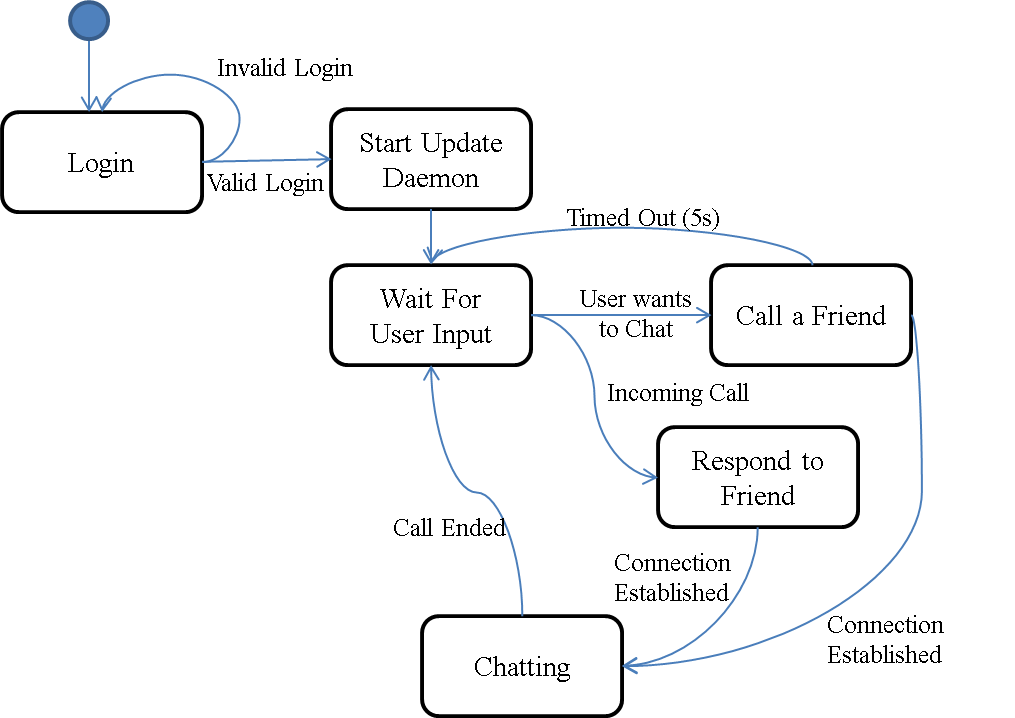
\includegraphics[width=0.8\textwidth]{pics/Client_StateDiagram}
   \caption{Client State Diagram demonstrating the general flow on the client-side.}
\label{fig:client_state_diag}
\end{figure*}

The client application is the core of the voice chatting system.  It initiates all
the communication with the server in order to receive the user's personal 
information which includes a friends list. For purposes of this paper, a friend
is one whom appears on the list of people a user can call. The application currently
does not support the ability for users to add friends during run-time.  Once the 
user logs into the server,
the client has free roam to make outgoing calls or answer incoming calls.  This
application only supports one-to-one chatting with a notification system that 
indicates when a friend is calling while the user is chatting with another client.  

The client-side of the system handles all the audio transmission between clients
as well as manages the setup and teardown of the transport protocol used to
communicate between two clients.  Each client is fitted with a transport protocol
object that handles all the layer three calls which send and receive data between
two clients using sockets.  The specific transport layer protocol is determined
upon loading the application by the user where DCCP, UDP, and TCP are the three
options. Each client is capable of calling friends as well as accepting calls from
other clients.  This requires a \textit{server} and \textit{client} model present
on each client's machine in order to monitor a socket for incoming calls as well
as open a new socket for outgoing calls.  Fig.~\ref{fig:client_state_diag} gives 
a state diagram representation of the client-side system.


The client communicates with the server once upon logging into the system and again
every time a client wants to call a friend.  When making an outgoing call,
the client asks the server for the hostname and port number of the friend he or
she wants to call.  This information is relayed back to the requestor which is then
used to directly call the friend of interest.  Since all communication with the
server contains important information about how to contact others within the 
network, the connection needs to be reliable; therefore, TCP is used for all 
communication between the clients and the server. Additionally, a seperate thread
is started immediately after logging into the server that handles receiving
periodic messages from the server which indicate any changes in the user's friends'
statuses. 


\subsection{Transport Layer Abstraction}
\label{subsec:transport_abs}

The main feature of this voice chatting application is its ability to easily 
swap in and out different transport layer protocols.  Essentially, this application
is a framework for testing the behavior of transport layer protocols with an
audio streaming application.  The abstraction was designed using the concept of
polymorphism.  Basically, a class called \textit{TransProtocol} was constructed
with several virtual functions that inhereting children must implement, i.e. DCCP,
TCP, and UDP.  These include the following:

\begin{itemize}
   \item{initMaster(uint16\_t)}
   \item{initSlave(char *, uint16\_t)}
   \item{sendPacket(void *, size\_t)}
   \item{recvPacket(void *, size\_t, int flags)}
   \item{getCallerID()}
   \item{ignoreCaller()}
   \item{answerCall()}
   \item{endCall()}
\end{itemize}

The above functions need to be implemented individually according to the specific
transport layer protocol.  For example, DCCP and TCP are connection-oriented and
need to setup a connection between two computers initially before any data packets 
can be transmitted whereas UDP connections open a socket and wait for 
whomever decides to send data its way.  The initialization steps for each of the
different transport layer protocols occur in the functions \textit{initMaster} and
\textit{initSlave}.  These two functions differ in the way the sockets are handled.

For the \textit{initMaster} function, the socket is bound to a randomly selected 
port in the same manner as the server does in a traditional server-client TCP model.
This port is then configured to listen for incoming requests. 
Before any clients can call this user, the port number needs to be reported to
the central server which saves it to a database. This port is continuously 
monitored by the client to notify the user of any incoming calls.  When an incoming
call is detected, the client machine accepts the call and extracts the caller's 
identification from the first packet to determine who the caller is using the 
\textit{getCallerID} function.  At this point, the user is notified when an 
incoming request has been received and is given the option to accept or decline
the call.  The appropriate action is taken based on the users response.

The \textit{initSlave} function is used when a client wants to make an outgoing
call to a friend.  For this to occur, the client machine requests from the central 
server the hostname and port number of the friend he or she wants to call 
identified by the user identification number.  After retrieving the proper contact 
information from the central server, \textit{initSlave} opens a socket to 
communicate with the friend.  Similar to the \textit{initMaster} function, if the
callee accepts the users call, then the chatting state will be entered and audio
capturing and playback will begin while being transferred across the transport
layer protocol of choice.

To handle processing the audio transmission and incoming chatting requests, the
main application was multi-threaded using boost threads.  Basically, the main
application thread handles the incoming requests and parses through the first
incoming request packets to identify who the caller is.  Once a connection
is established between two clients and the callee accepts the call, a chatting
thread is spawned that handles the audio capturing and playback along with the 
packet construction and transmission.  Within the chatting thread, there is an
audio playback thread started, which is discussed in the next section.


\subsection{Audio Processing}
\label{subsec:audio_proc}

Audio transmission was handled in the simplest possible manner.  The ALSA libraries
were used to capture and playback the raw audio from the microphone on each of the 
client's machines.  The ALSA libraries were used because of their simplicity and
built-in linux functionality.   

The audio was captured at 8,000 bytes per second on 2 channels.  In a 
single packet, 1,400 bytes are transmitted.  The capture and transmission of audio 
data occurs in the main chatting thread while the playback of the received audio 
packets occurr in a seperate thread.  This thread is dedicated to reading from
a buffer that contains received audio packets.  To reduce the latency 
introduced by transmitting in real-time over a network, a minimum buffer size
threshold was set to 5 packets.




\section{Evaluation}

\subsection{Experiment Setup}

Our experiments were conducted on a small LAN consisting of two laptops and two
workstations in the networks lab, all of which were connected by a small 10 Mbit
Ethernet hub. The lab workstations each ran an iperf client and an iperf server
in UDP mode, while our laptops each ran our chat client along with Wireshark.
One of our laptops also ran our chat server. Figure~\ref{fig:test_network} shows a
diagram of our test network.

\begin{figure*}[!t]
   \centering
      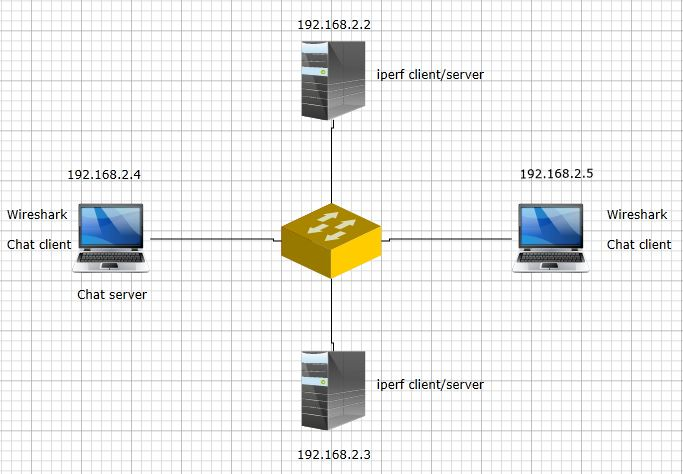
\includegraphics[width=0.7\textwidth]{pics/network_diagram}
   \caption{Test network diagram.}
\label{fig:test_network}
\end{figure*}

\subsection{Experiment Procedure}

Each of our test runs was conducted as follows. First, we started the iperf
clients and servers on the lab workstations and configured the clients to
generate the desired level of background traffic. Since both workstations were
running iperf clients, this resulted in cross-traffic flowing between the two
workstations. After initializing iperf, we started Wireshark captures on both of
our machines. We then initiated a call between our chat clients, let the call
continue for 30 seconds, then aborted the call and saved both Wireshark captures. We
tested each protocol with the iperf clients sending 0, 9, and 10 Mbit/s of
traffic, and each run was repeated a total of five times.

\subsection{Analysis Procedure}

In order to calculate packet losses, we used the Wireshark traces captured
during our experiments to determine how many packets were sent from one client
and received by the other. Specifically, we did this by applying this display
filter to both Wireshark traces from a particular session:

\texttt{(dccp|tcp|udp) and ip.src == 192.168.2.5 and data.len == 1407}

For the first term, we used the name of the protocol being used by our chat
program when the traces were captured. This expression filtered out all packets except data packets that were sent from
192.168.2.5, one of our laptops. For the trace recorded on 192.168.2.5, the
number of displayed packets told us how many packets were sent from 192.168.2.5.
Similarly, for the trace recorded on 192.168.2.4 (that is, the other chat
client), only data packets received from 192.168.2.5 were displayed. We
calculated the number of lost packets as the difference between these two
numbers.

We did not have a good way to directly measure network latency during our
experiments. Therefore, in order to analyze jitter, we measured delays between
incoming data packets. For each of our runs, we calculated the average delay
between consecutive pairs of incoming packets, and then calculated jitter as the
difference between an individual delay and the average delay. Finally, we
graphed the resulting jitter measurements as CDFs, with jitter on the X-axis and
the associated percentiles on the Y-axis.

\subsection{Discussion}

\subsubsection{Losses and Sending Rates}

As previously stated, we computed packet losses for each run. Our results are
shown in Figures ~\ref{fig:avg_losses}, ~\ref{fig:dccp_losses},
~\ref{fig:tcp_losses}, and ~\ref{fig:udp_losses}.

Unfortunately, our chat client proved unstable and crashed multiple times during
our UDP test runs. In an attempt to work around the issue, we tried starting our
Wireshark captures after initializing the voice call and the iperf clients. We
tried to synchronize the start of our captures, but a handful of our UDP
captures were nevertheless out of sync and yielded invalid loss data. This is
why we have no packet loss data for UDP session 3 at 9 Mbit/s background
traffic. We acknowledge this was hardly an ideal solution, but we were unable to
troubleshoot the chat client effectively due to lack of time and one of our
group being unavailable for later stages of testing.

It is interesting to note that, on average, DCCP dropped approximately 5\% more
packets at 9 Mbit/s of background traffic compared to 10 Mbit/s, whereas TCP
lost more packets at 10 Mbit/s than at 9 Mbit/s. Our program uses DCCP's
CCID2 congestion control mechanism, which is quite similar to TCP's congestion
control, so we are not sure why the two protocols appeared to behave differently
in this regard. Since this result seems counter-intuitive and the observed
difference is small, we believe it is most likely due to another factor not
under our control.

\begin{figure}[!h]
   \centering
      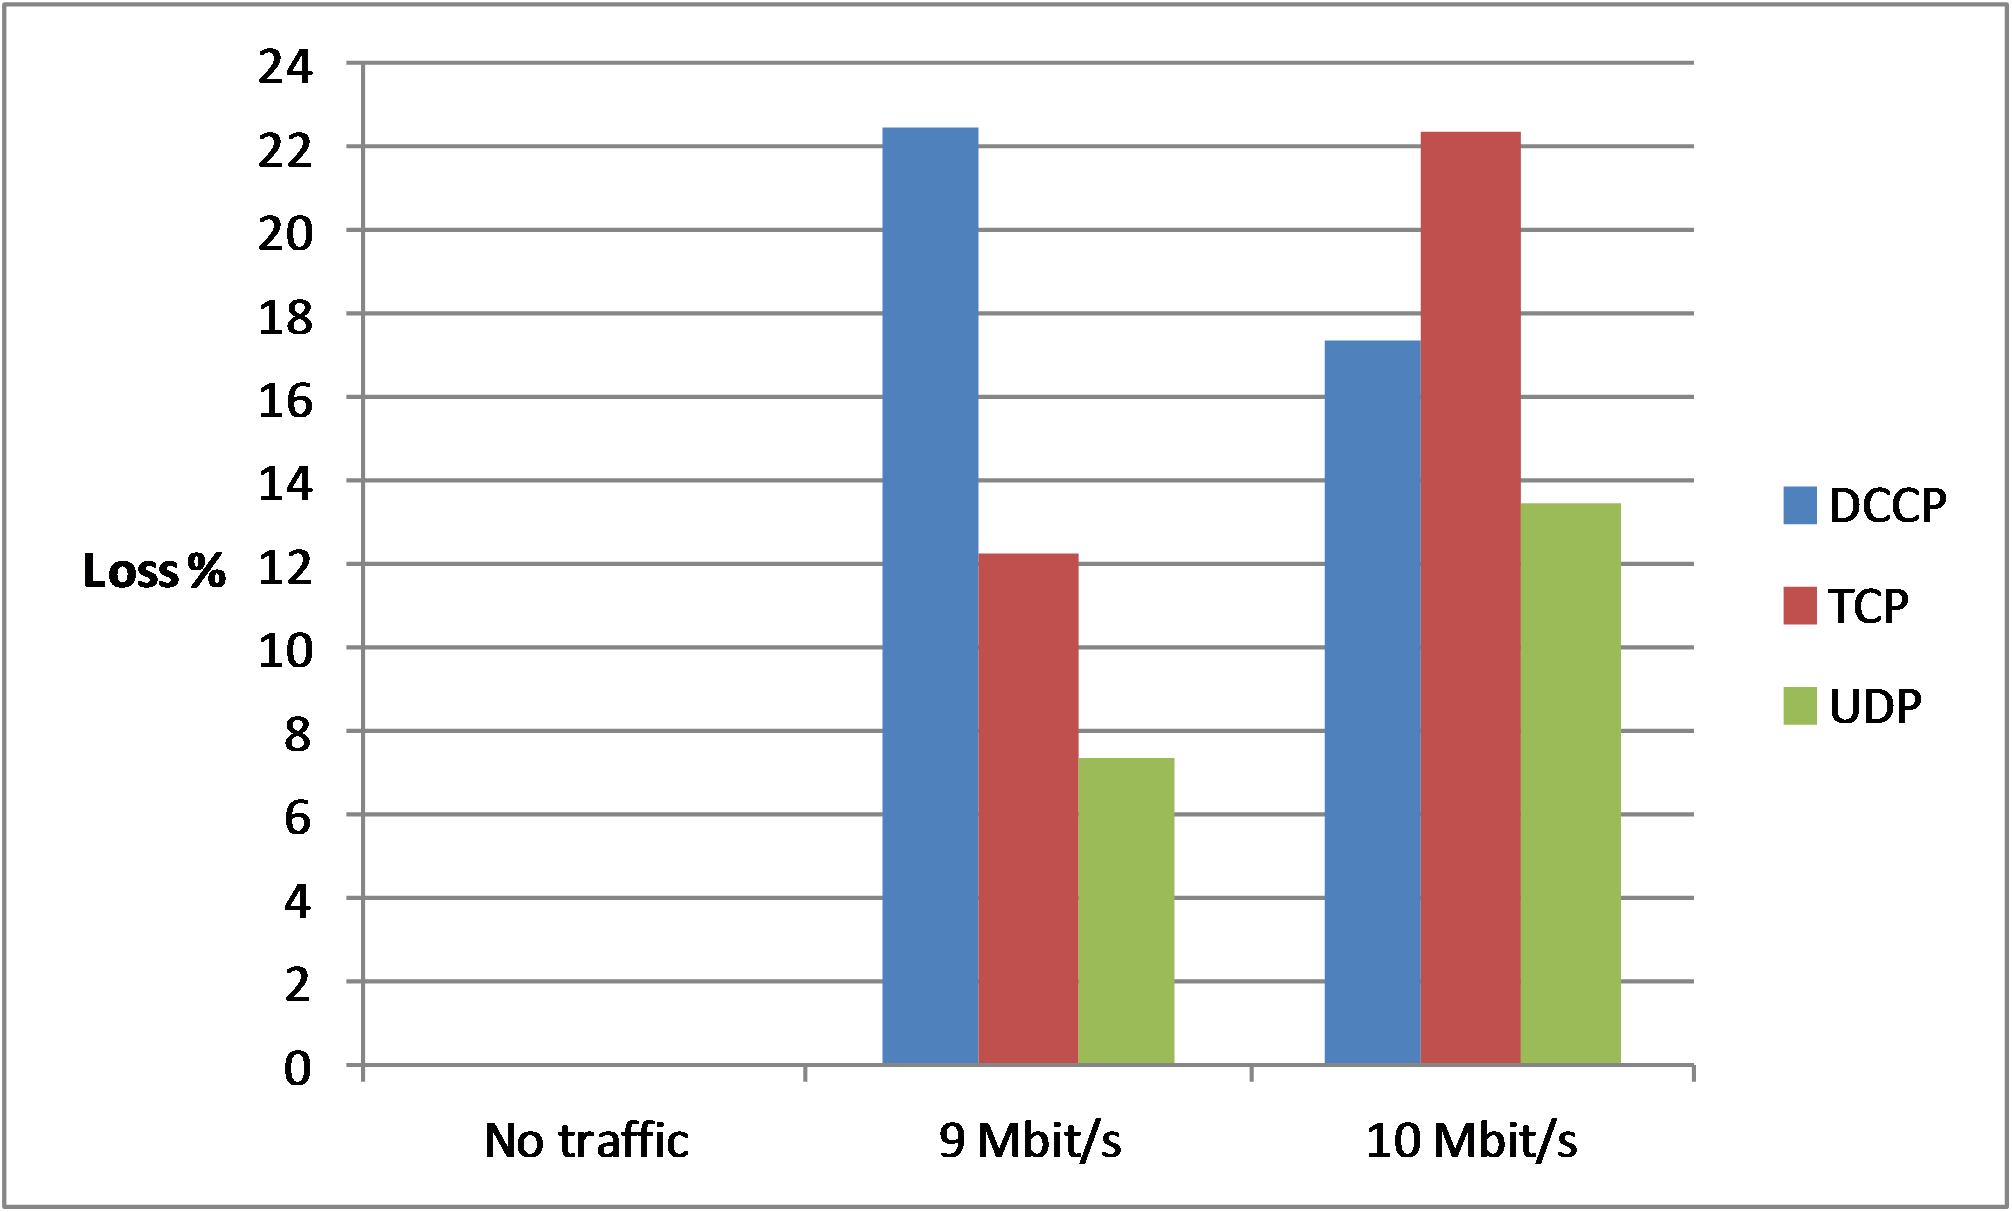
\includegraphics[width=0.45\textwidth]{pics/avg_losses}
   \caption{Average packet losses for each protocol.}
\label{fig:avg_losses}
\end{figure}

\begin{figure}[!h]
   \centering
      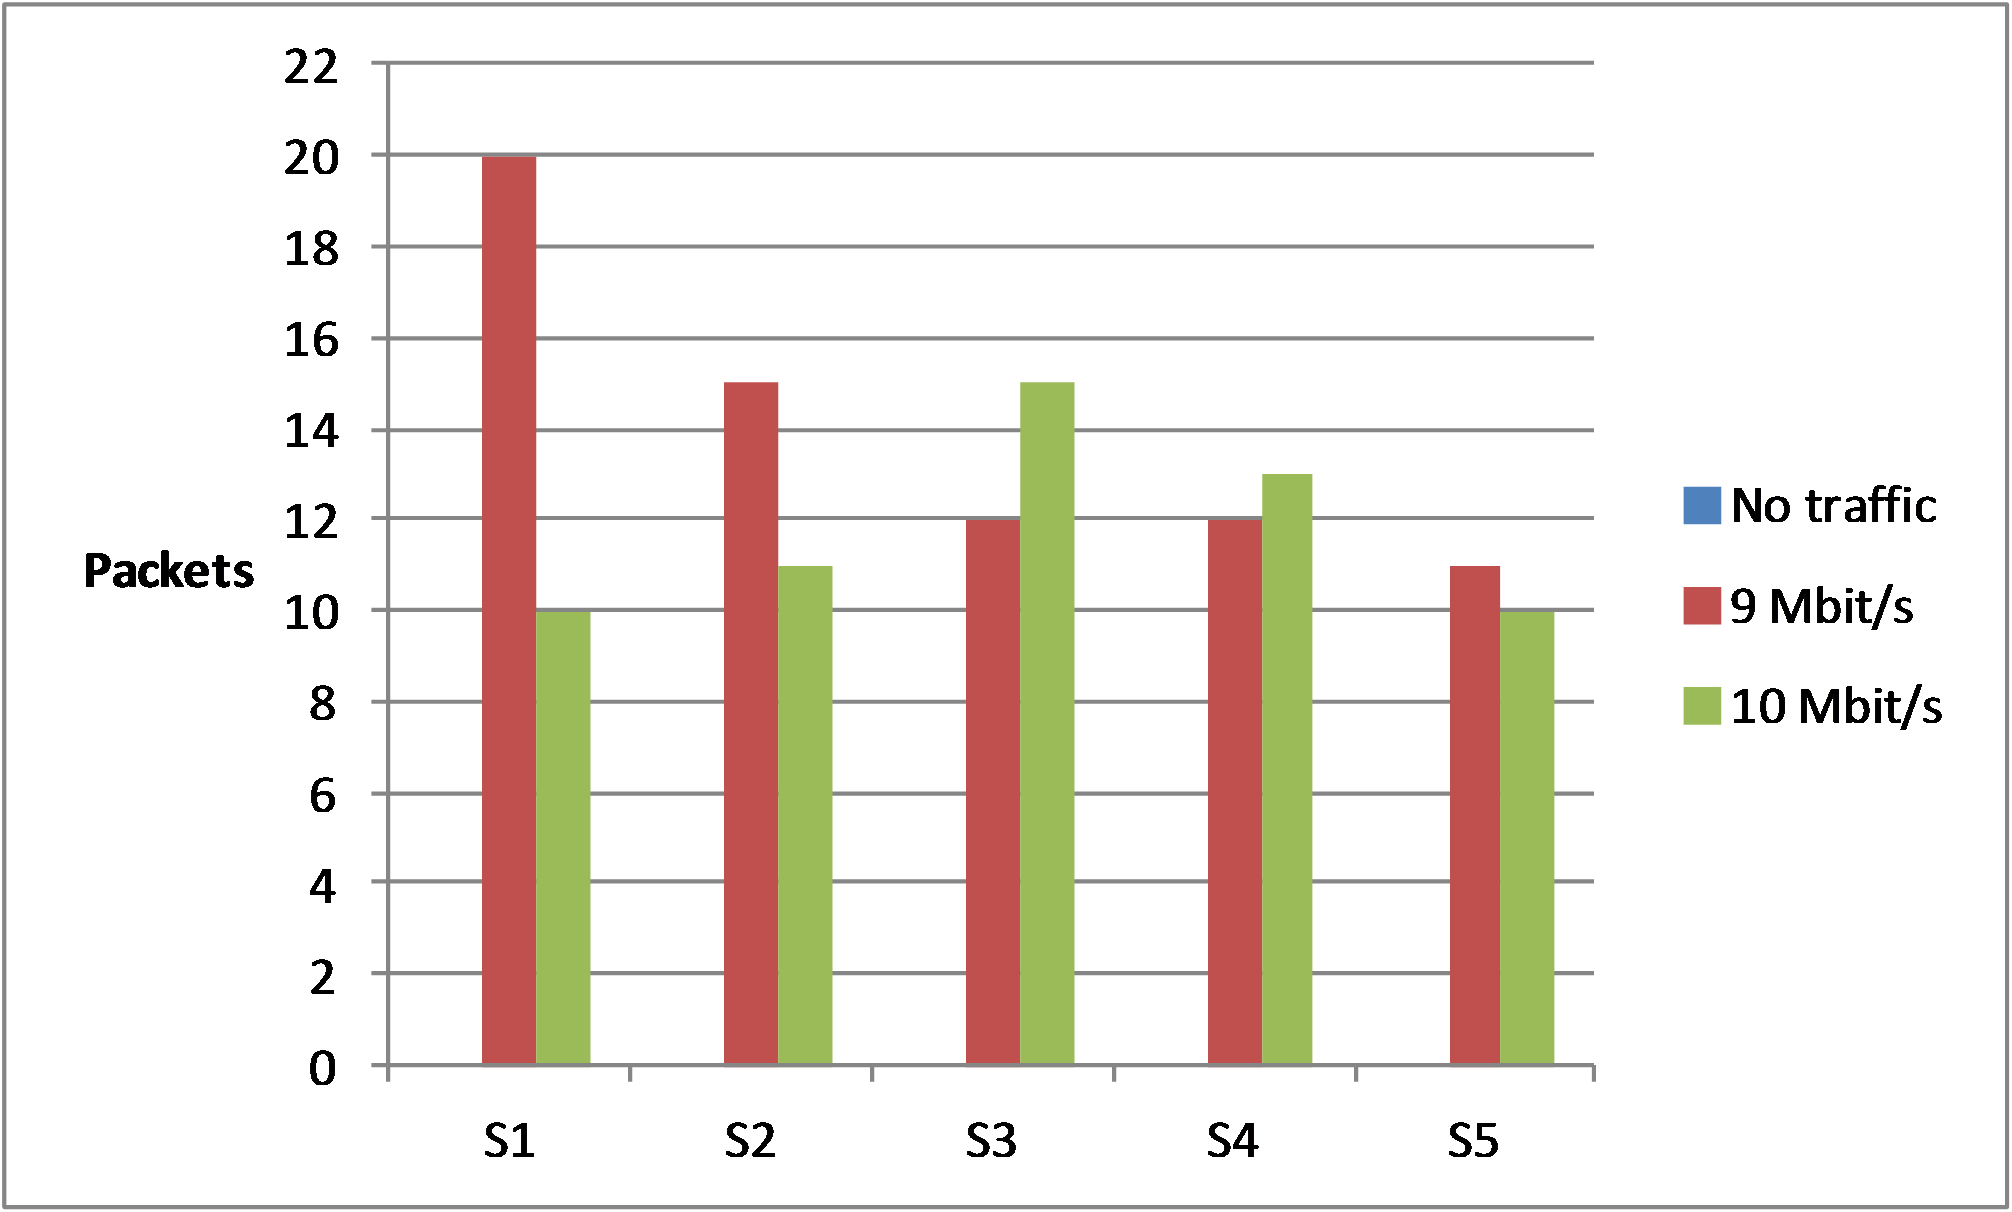
\includegraphics[width=0.45\textwidth]{pics/dccp_losses}
   \caption{Packets lost for all DCCP runs.}
\label{fig:dccp_losses}
\end{figure}

\begin{figure}[!h]
   \centering
      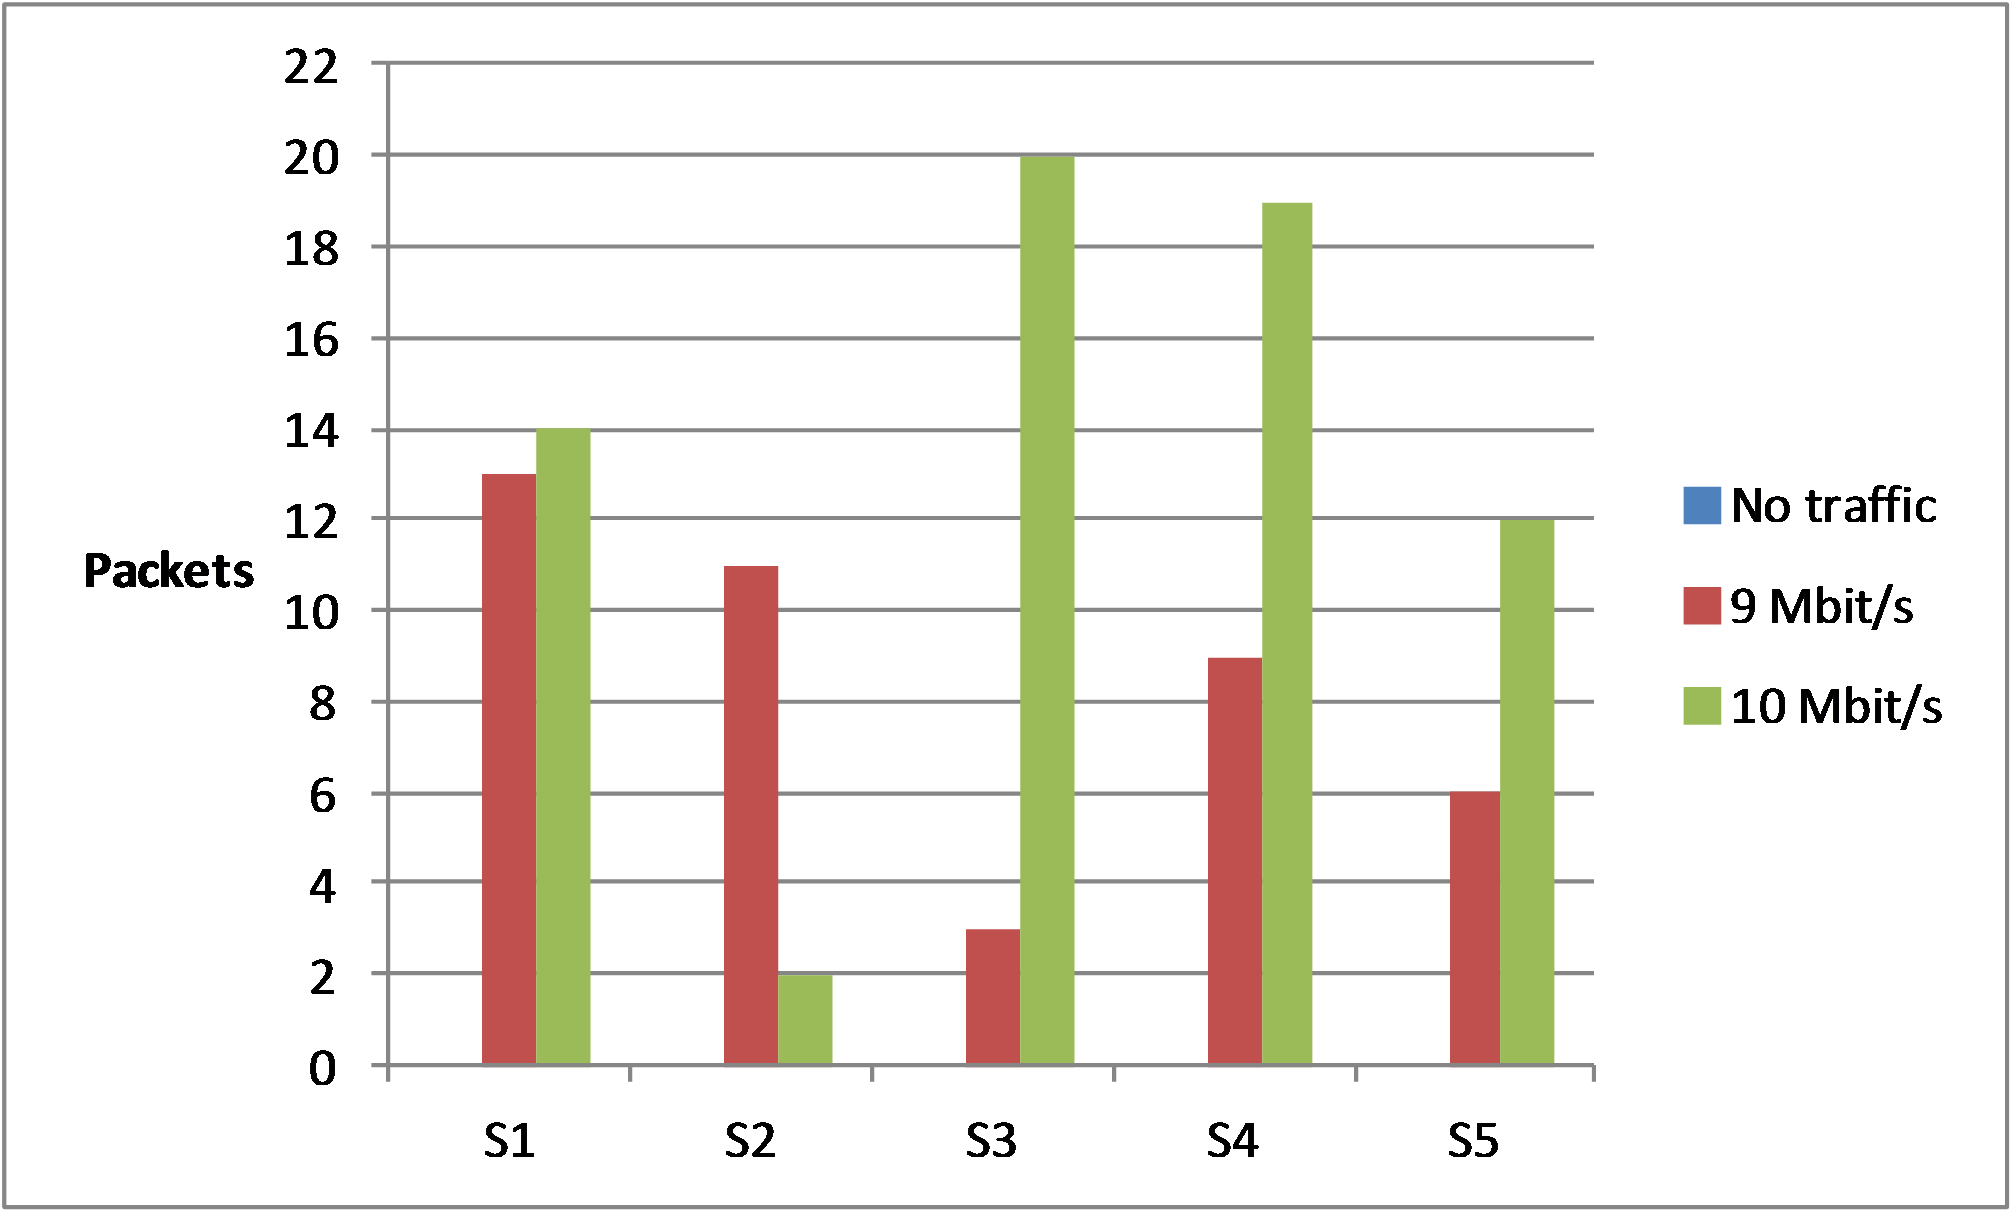
\includegraphics[width=0.45\textwidth]{pics/tcp_losses}
   \caption{Packets lost for all TCP runs.}
\label{fig:tcp_losses}
\end{figure}

\begin{figure}[!h]
   \centering
      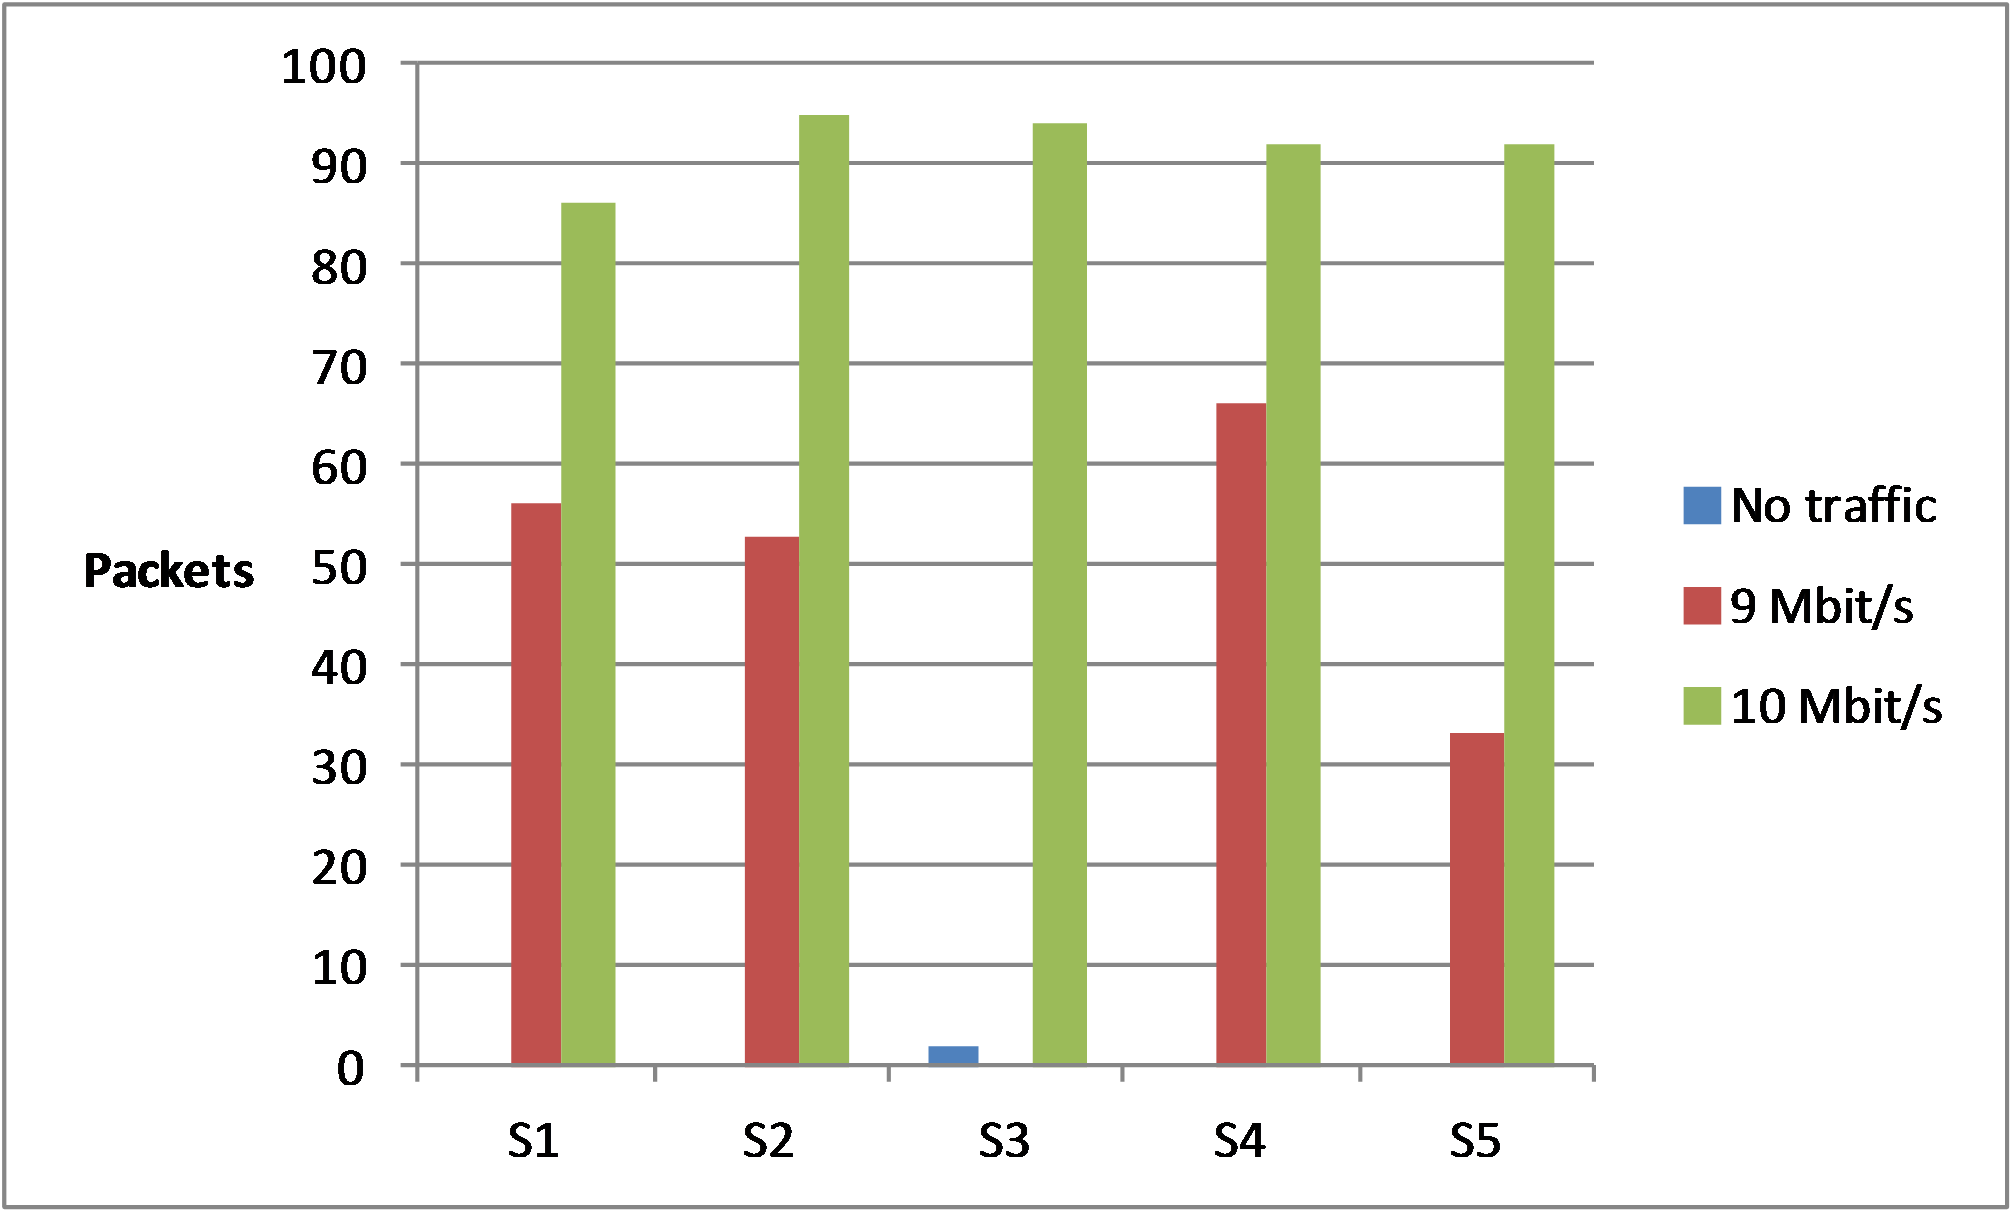
\includegraphics[width=0.45\textwidth]{pics/udp_losses}
   \caption{Packets lost for all UDP runs.}
\label{fig:udp_losses}
\end{figure}

Our experiments also allowed us to observe how each protocol throttled its
sending rate in response to increasing network congestion. Figures
~\ref{fig:dccp_sent},~\ref{fig:tcp_sent}, and~\ref{fig:udp_sent} give our
measurements.

As expected, DCCP and TCP transmit significantly fewer packets when congestion
is severe, but UDP continues to send approximately the same volume of packets
regardless of network conditions. In particular, TCP's behavior is extremely
regular, with each run producing very similar results. On the other hand, DCCP
demonstrated substantial variability in our tests with no background traffic.
Session 5 in particular showed a transmission rate comparable to that observed
during high congestion. However, since there was no other competing traffic on
the network during these tests, we do not believe the DCCP protocol itself is
responsible for this behavior. Rather, we believe the host machines' operating
system or a bug in our chat program may have sometimes caused a lower packet
volume.

\begin{figure}[!h]
   \centering
      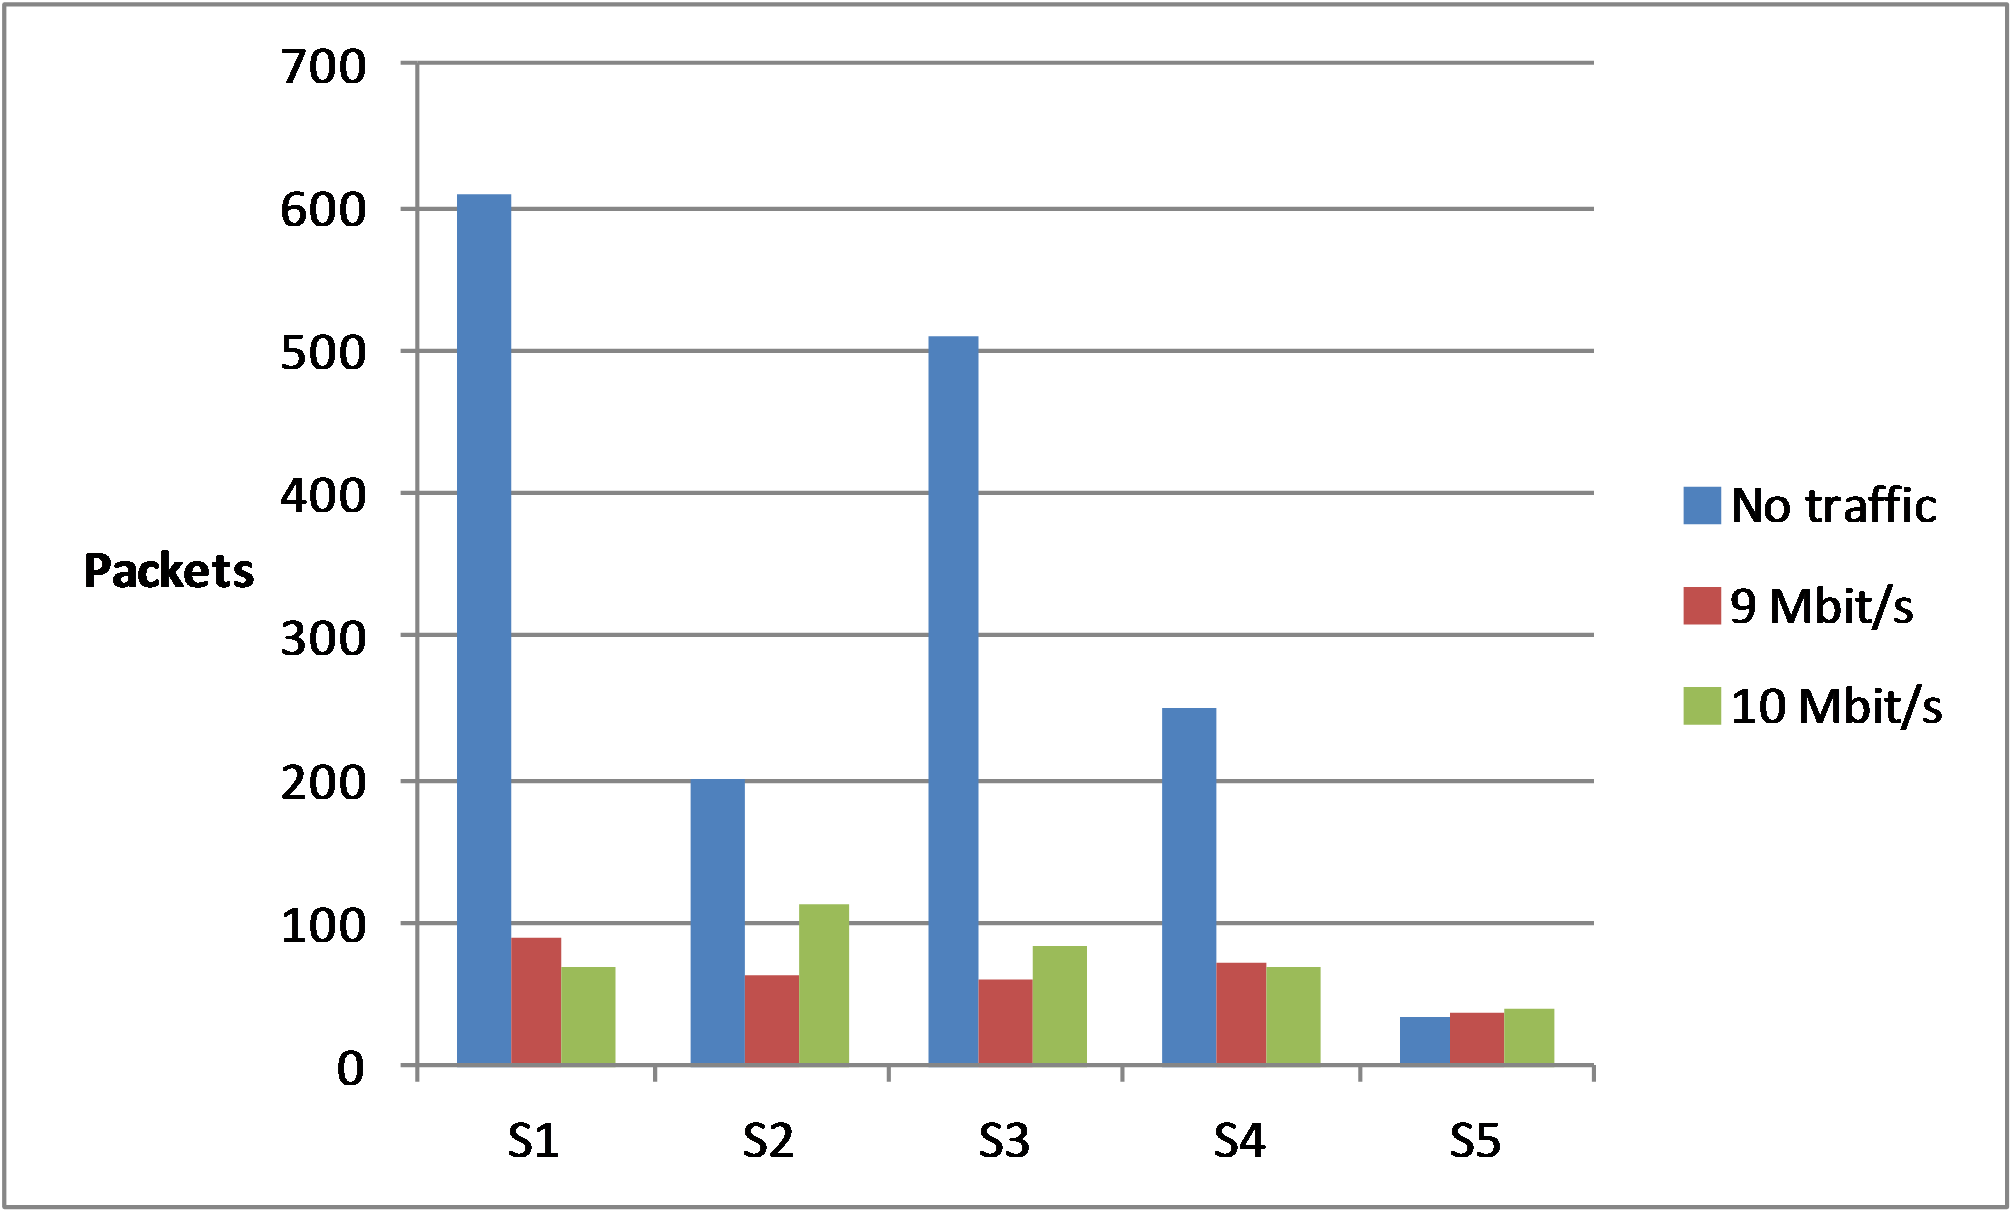
\includegraphics[width=0.45\textwidth]{pics/dccp_sent}
   \caption{Packets sent during all DCCP tests.}
\label{fig:dccp_sent}
\end{figure}

\begin{figure}[!h]
   \centering
      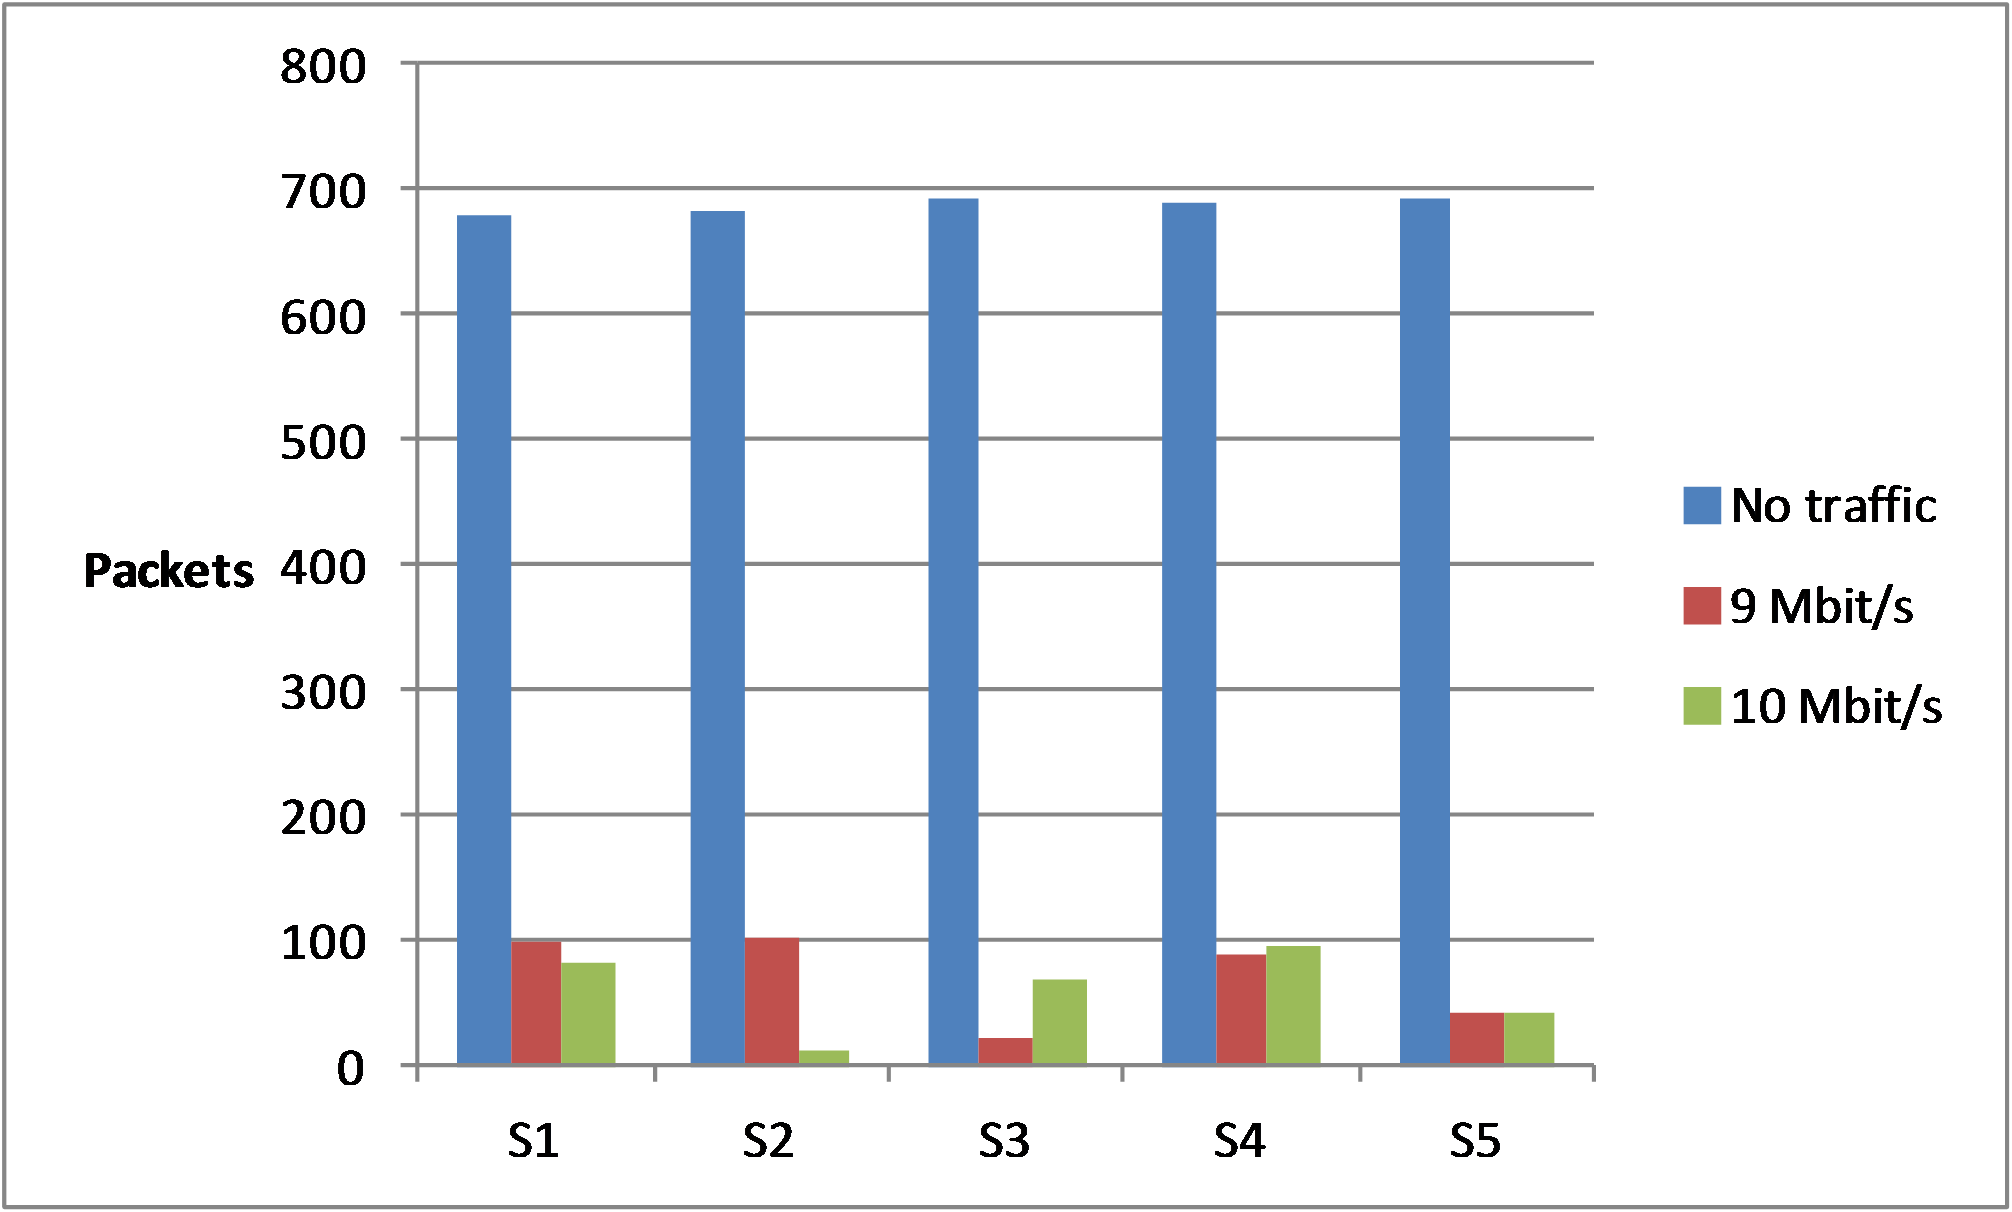
\includegraphics[width=0.45\textwidth]{pics/tcp_sent}
   \caption{Packets sent during all TCP tests.}
\label{fig:tcp_sent}
\end{figure}

\begin{figure}[!h]
   \centering
      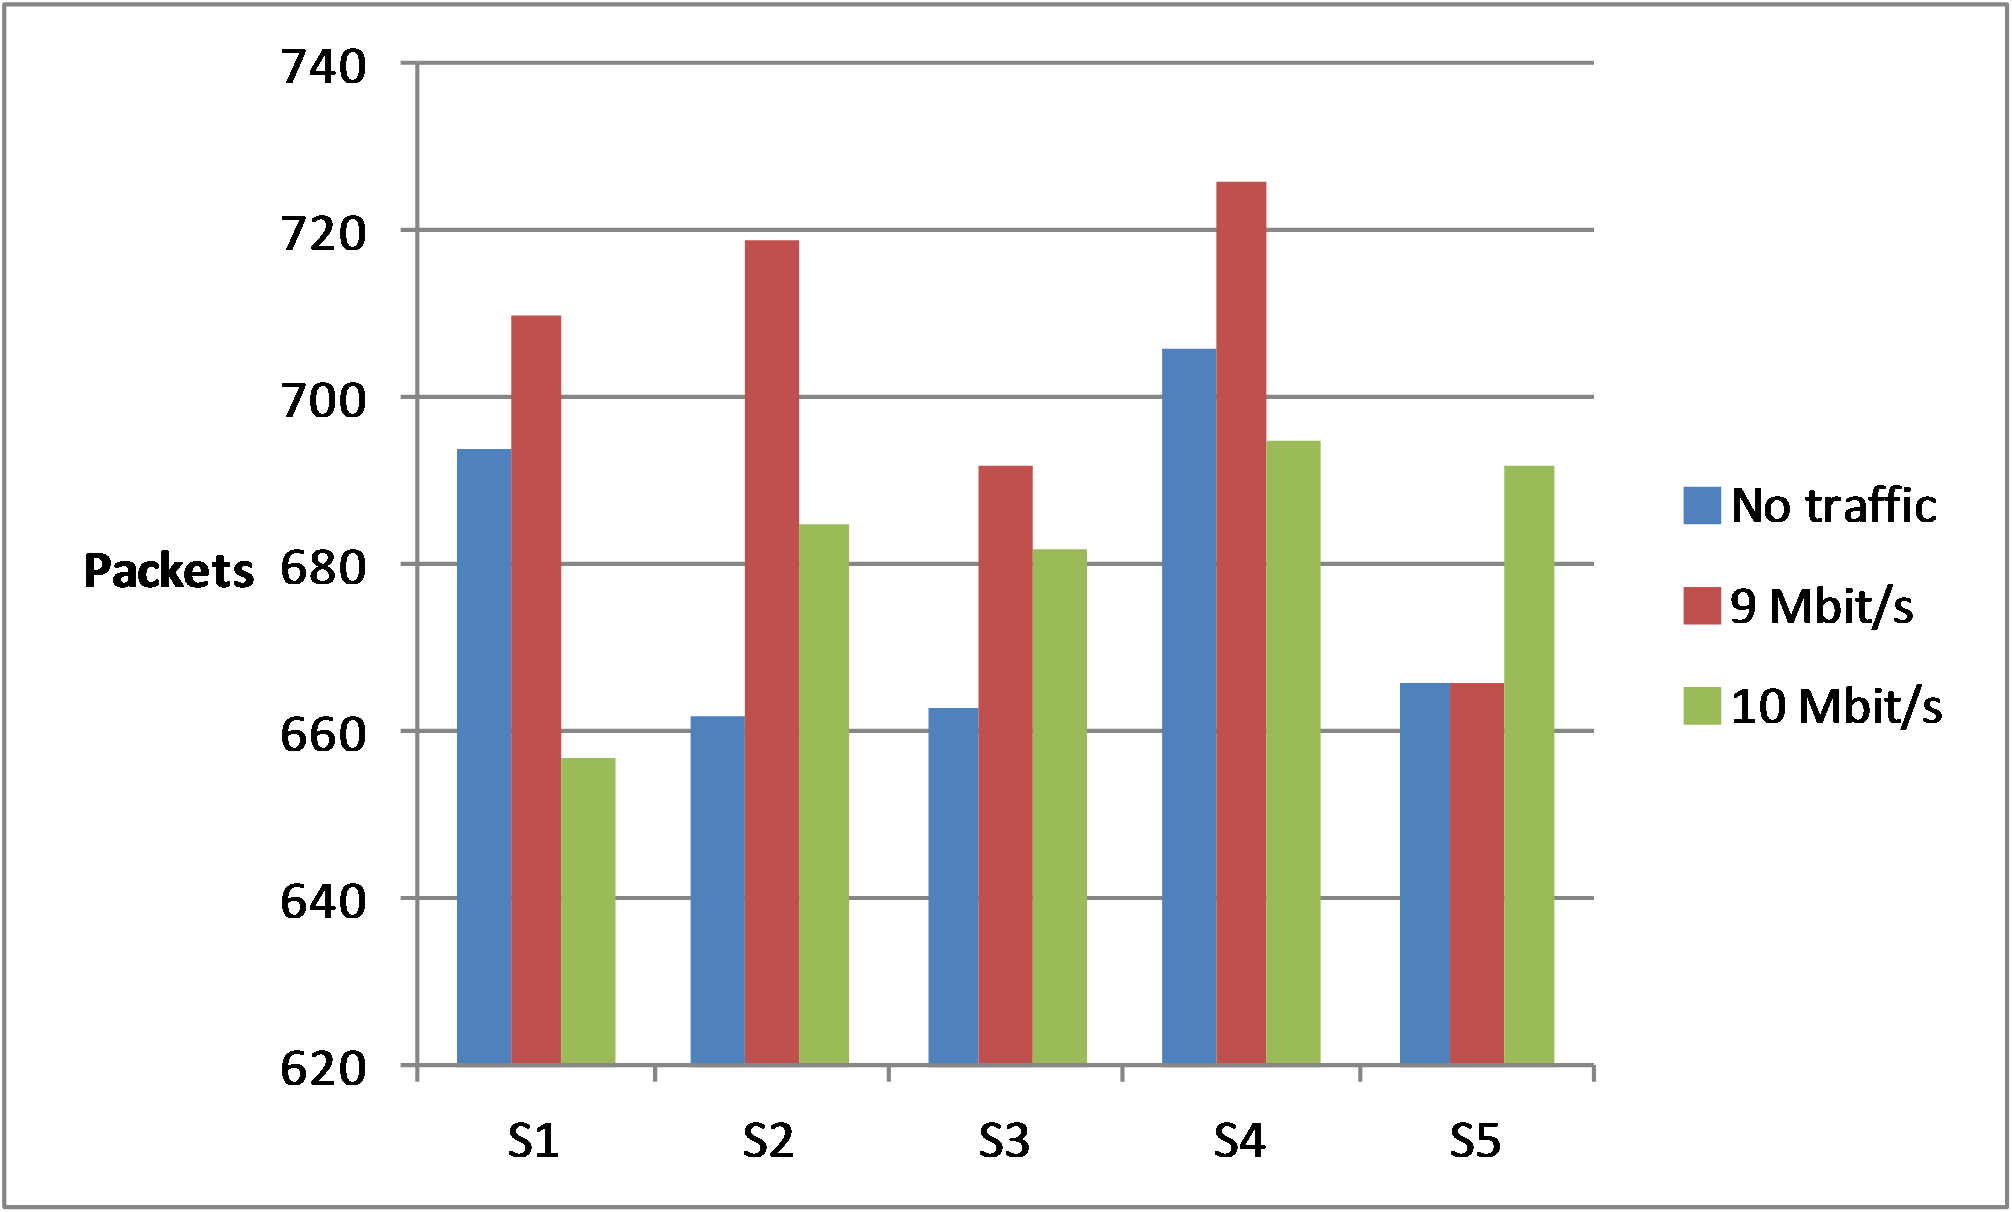
\includegraphics[width=0.45\textwidth]{pics/udp_sent}
   \caption{Packets sent during all UDP tests.}
\label{fig:udp_sent}
\end{figure}

\subsubsection{Jitter}

This section gives our jitter measurements for each protocol at each of our
three background traffic levels. Each graph seen in Fig.~\ref{fig:jitter_graphs} is a CDF of our aggregated jitter
measurements for each protocol and congestion level, convering all five
individual sessions. Figures ~\ref{fig:jitter_detail_9} and
~\ref{fig:jitter_detail_10} are CDF graphs for single protocols at each
congestion level. These figures have reduced X scales in order to better show
details of their jitter distributions.

\begin{figure*}[!t]
   \centering
   \subfloat[Jitter CDF with no background traffic.]{
      \label{fig:notraffic_jitter}
      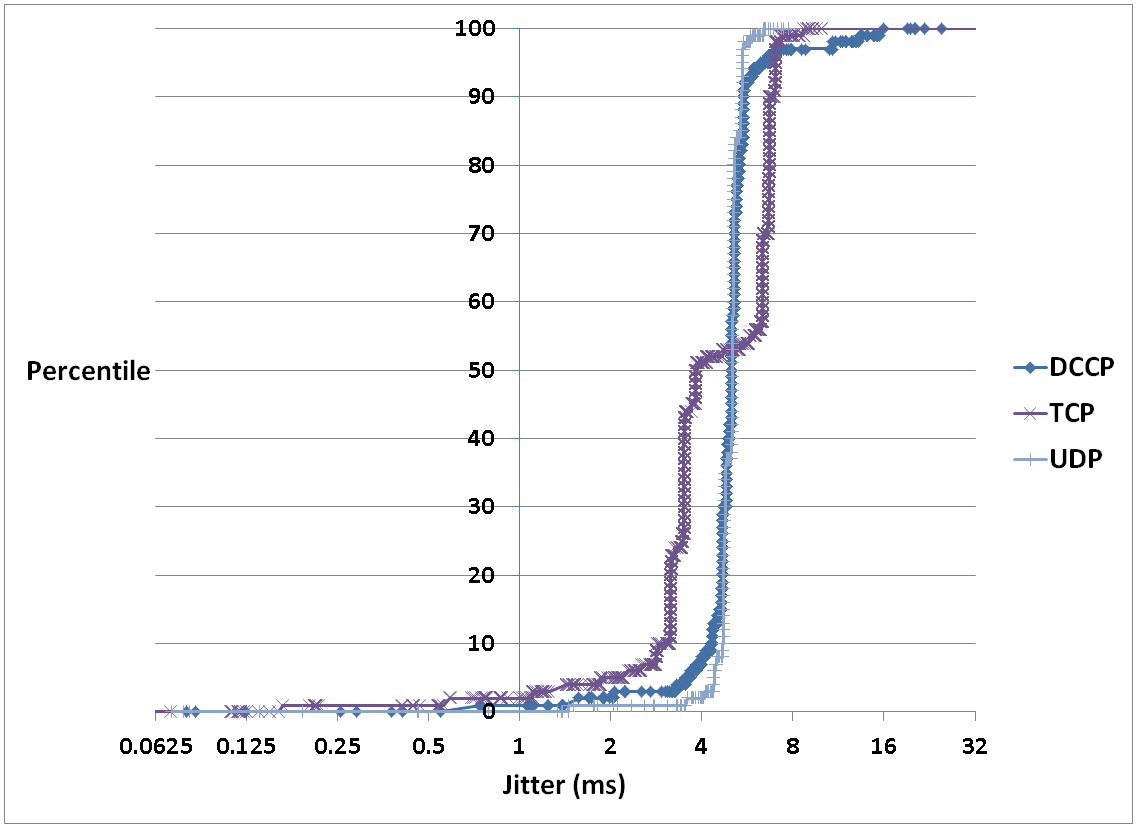
\includegraphics[width=0.45\textwidth]{pics/no_traffic_jitter}}
   \subfloat[Jitter CDF for 9 Mbit/s.]{
      \label{fig:9mbs_jitter}
      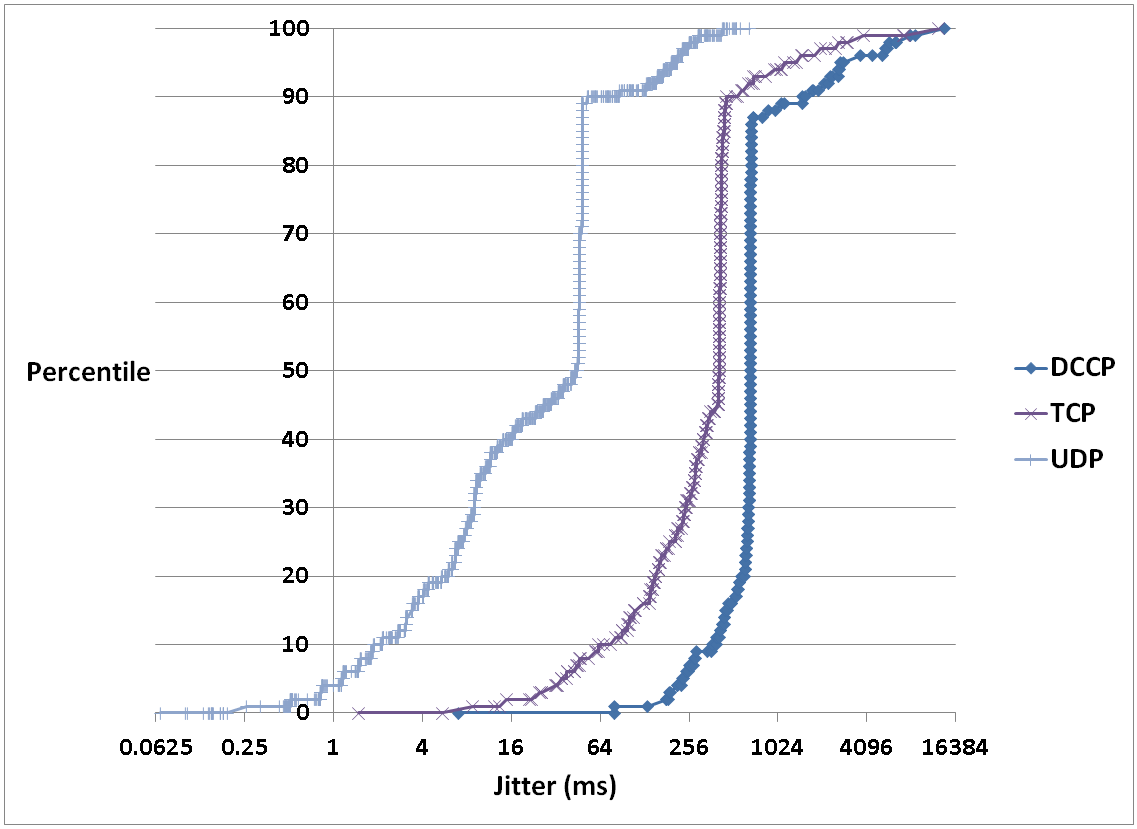
\includegraphics[width=0.45\textwidth]{pics/9mbs_jitter}}
  \\ \subfloat[Jitter CDF for 10 Mbit/s.]{
      \label{fig:10mbs_jitter}
      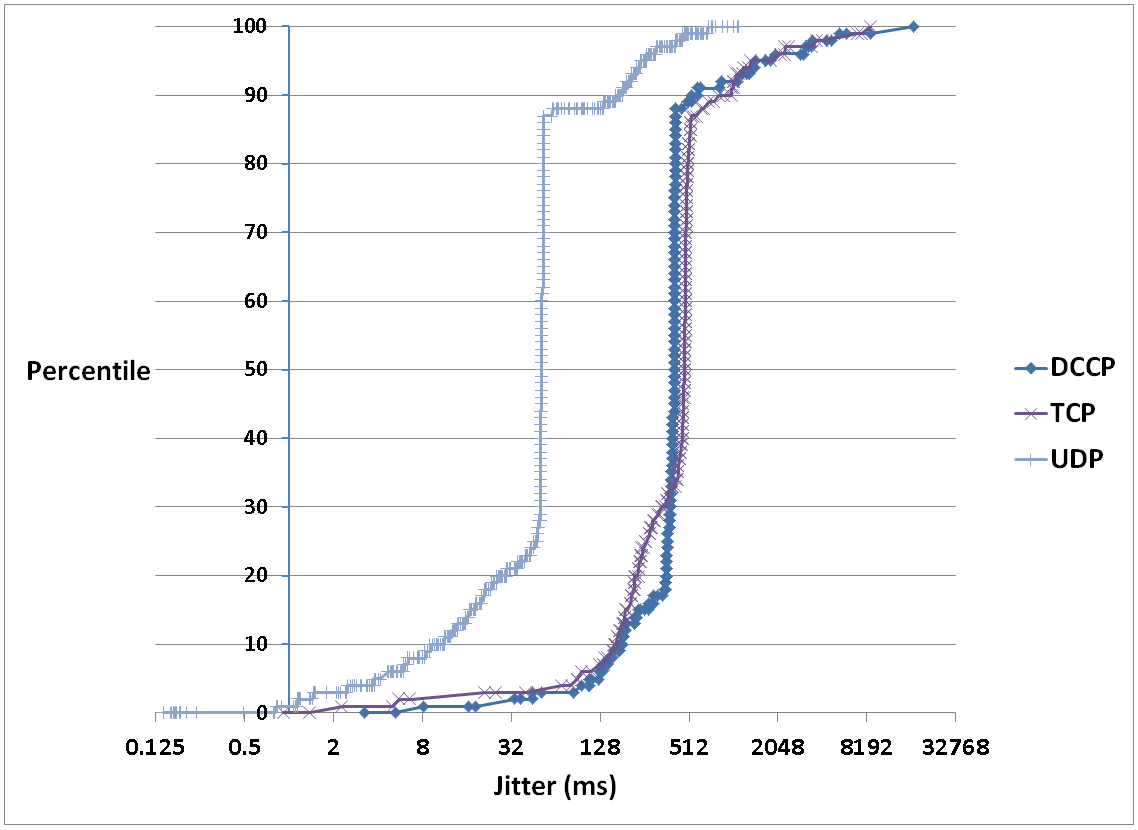
\includegraphics[width=0.45\textwidth]{pics/10mbs_jitter}}
   \caption{Jitter CDFs for three different extremes of background traffic.}
\label{fig:jitter_graphs}
\end{figure*}

\begin{figure*}[!t]
   \centering
   \subfloat[DCCP.]{
      \label{fig:dccp_9_jitter_closeup}
      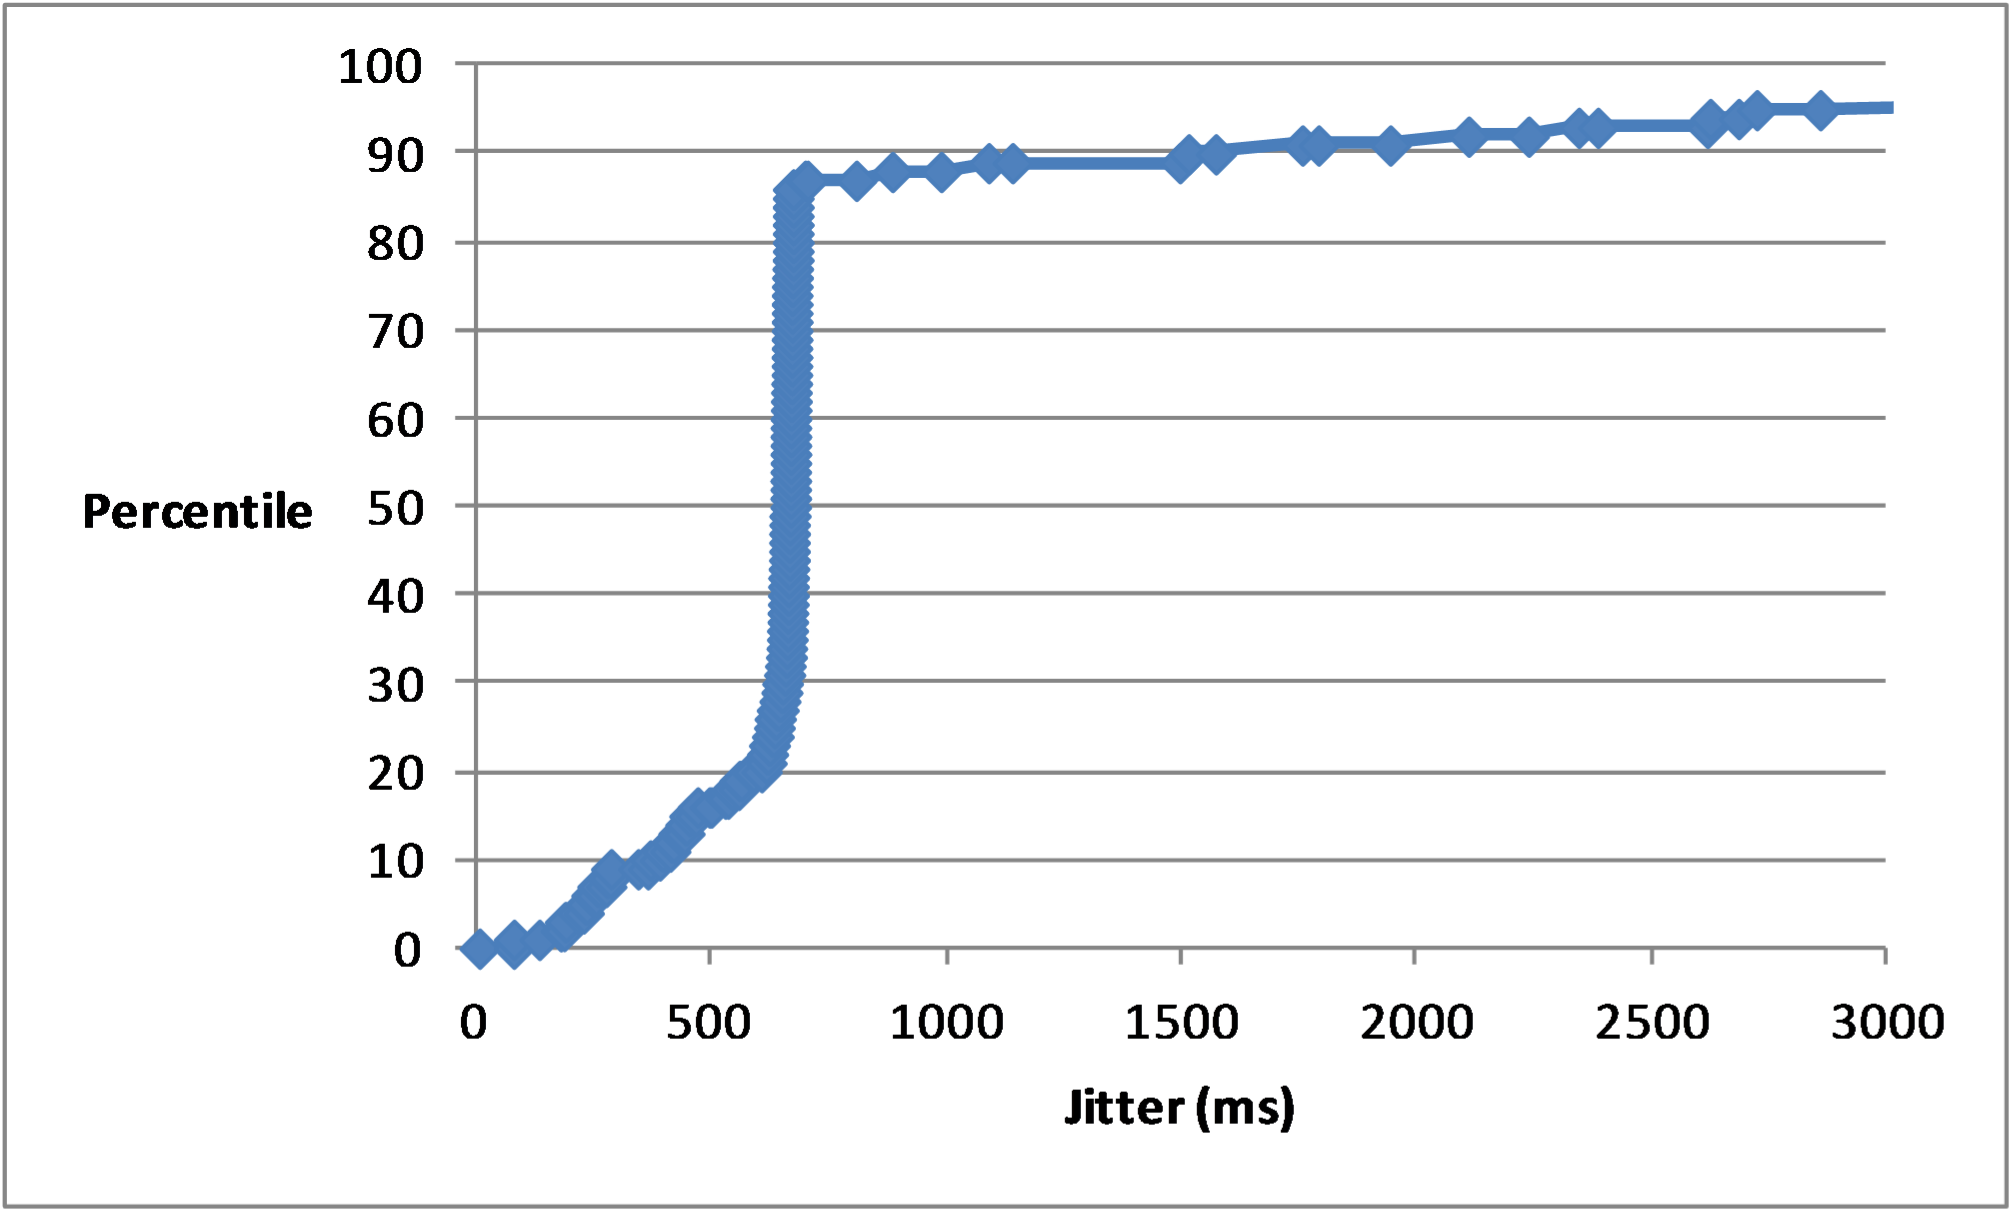
\includegraphics[width=0.45\textwidth]{pics/dccp_9_jitter_closeup}}
   \subfloat[TCP.]{
      \label{fig:tcp_9_jitter_closeup}
      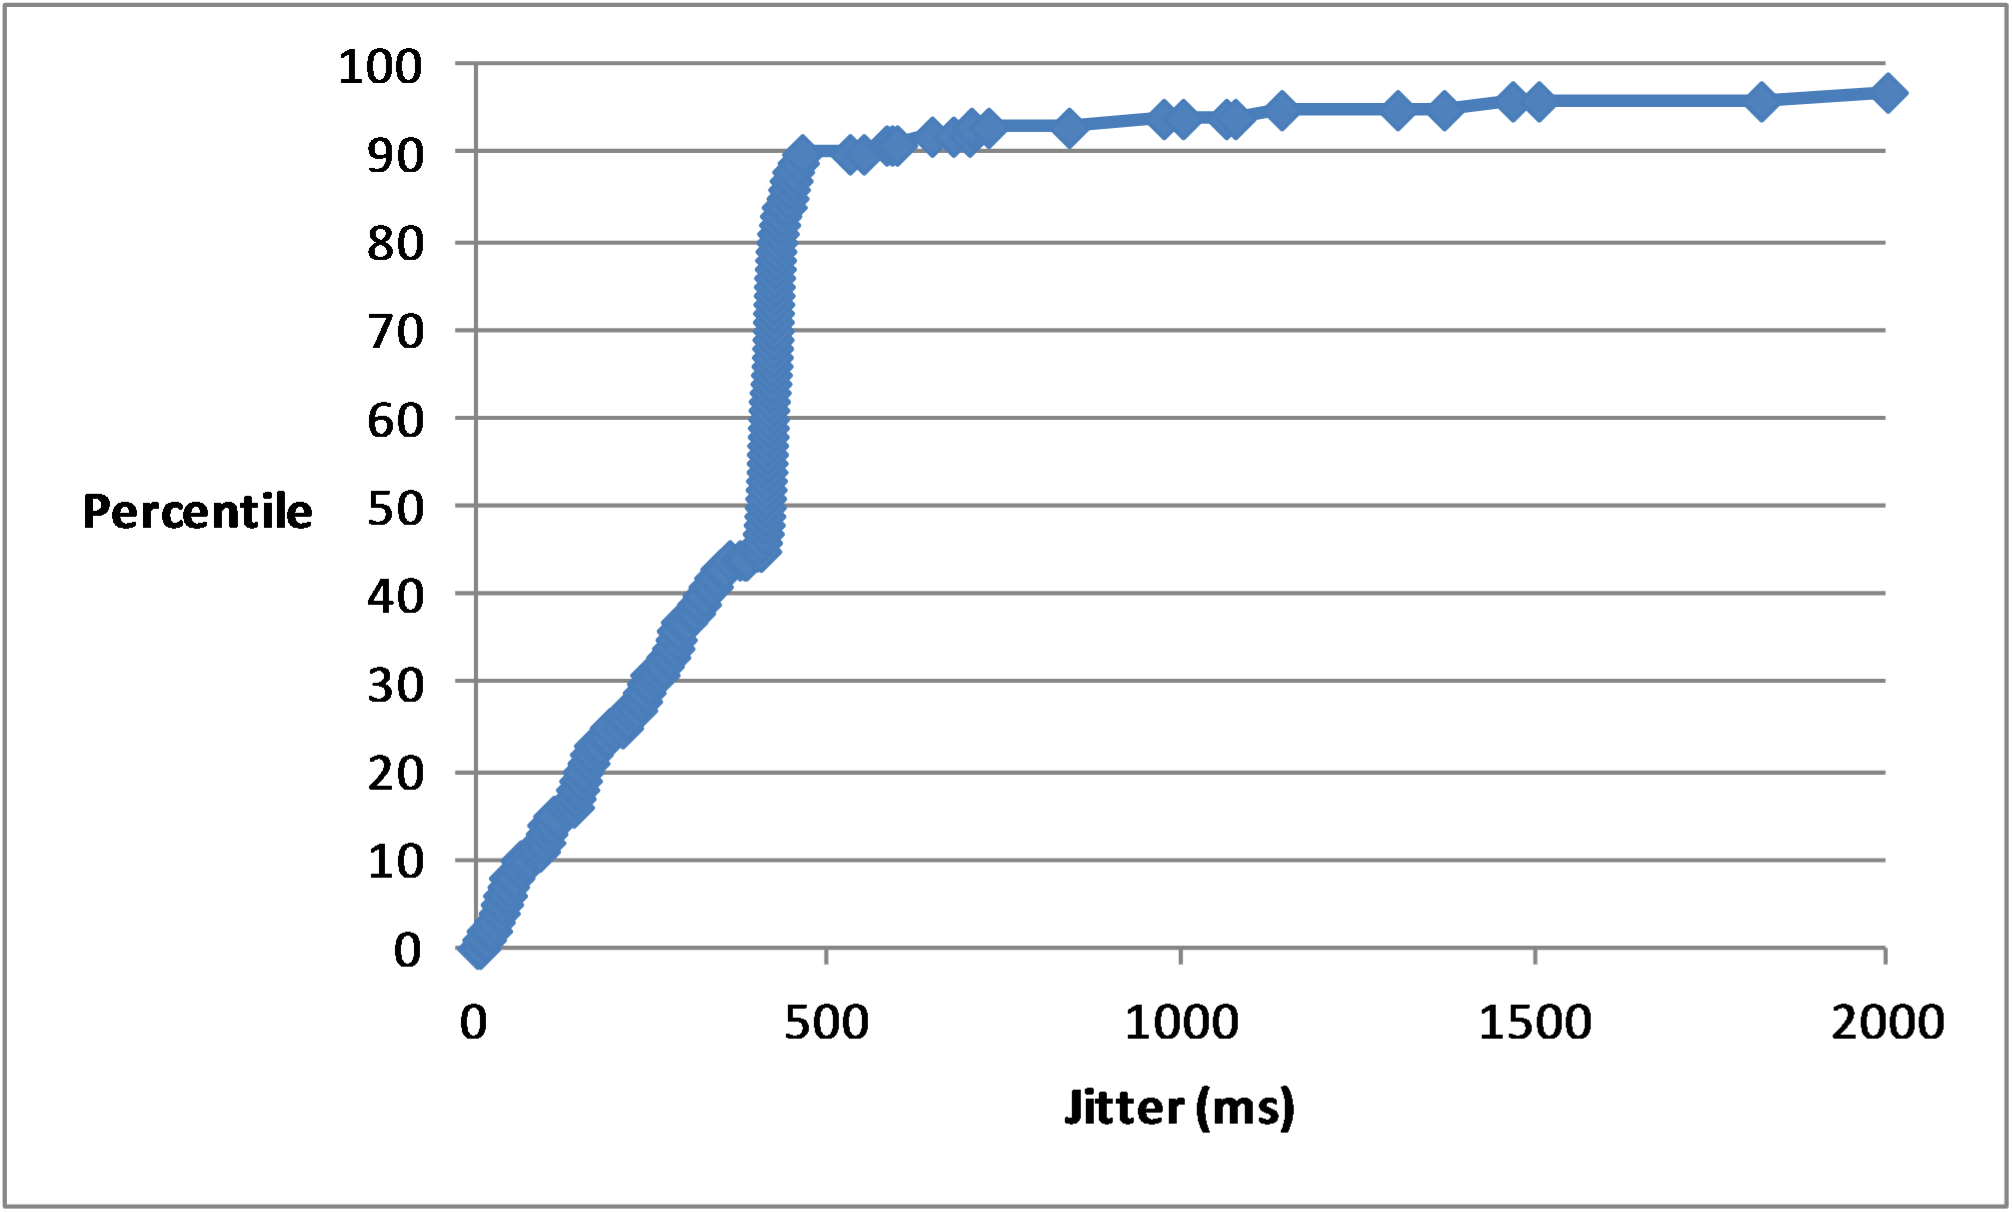
\includegraphics[width=0.45\textwidth]{pics/tcp_9_jitter_closeup}}
  \\ \subfloat[UDP.]{
      \label{fig:udp_9_jitter_closeup}
      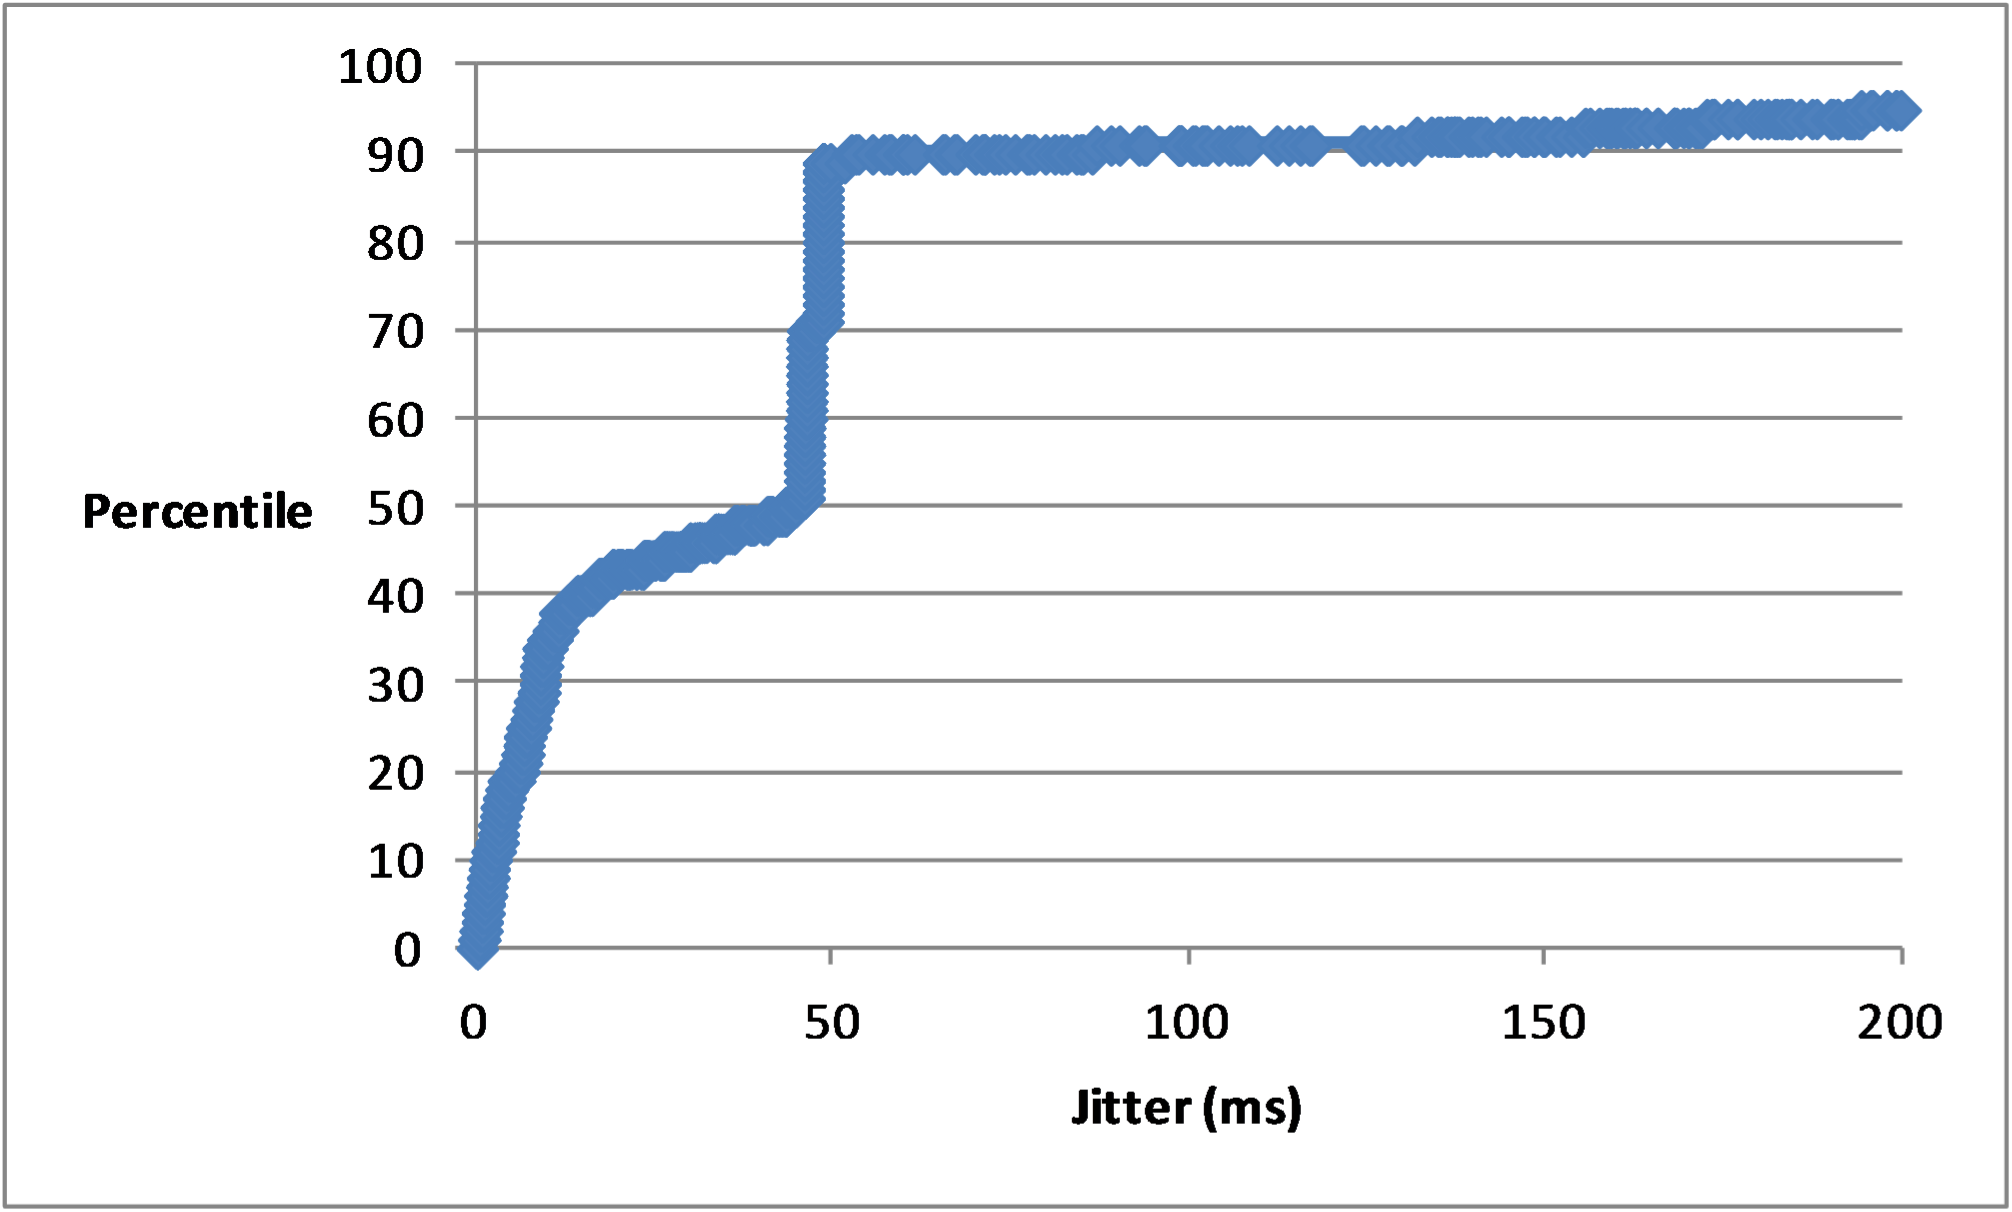
\includegraphics[width=0.45\textwidth]{pics/udp_9_jitter_closeup}}
   \caption{Detailed jitter CDFs for 9 Mbit/s.}
\label{fig:jitter_detail_9}
\end{figure*}

\begin{figure*}[!t]
   \centering
   \subfloat[DCCP.]{
      \label{fig:dccp_10_jitter_closeup}
      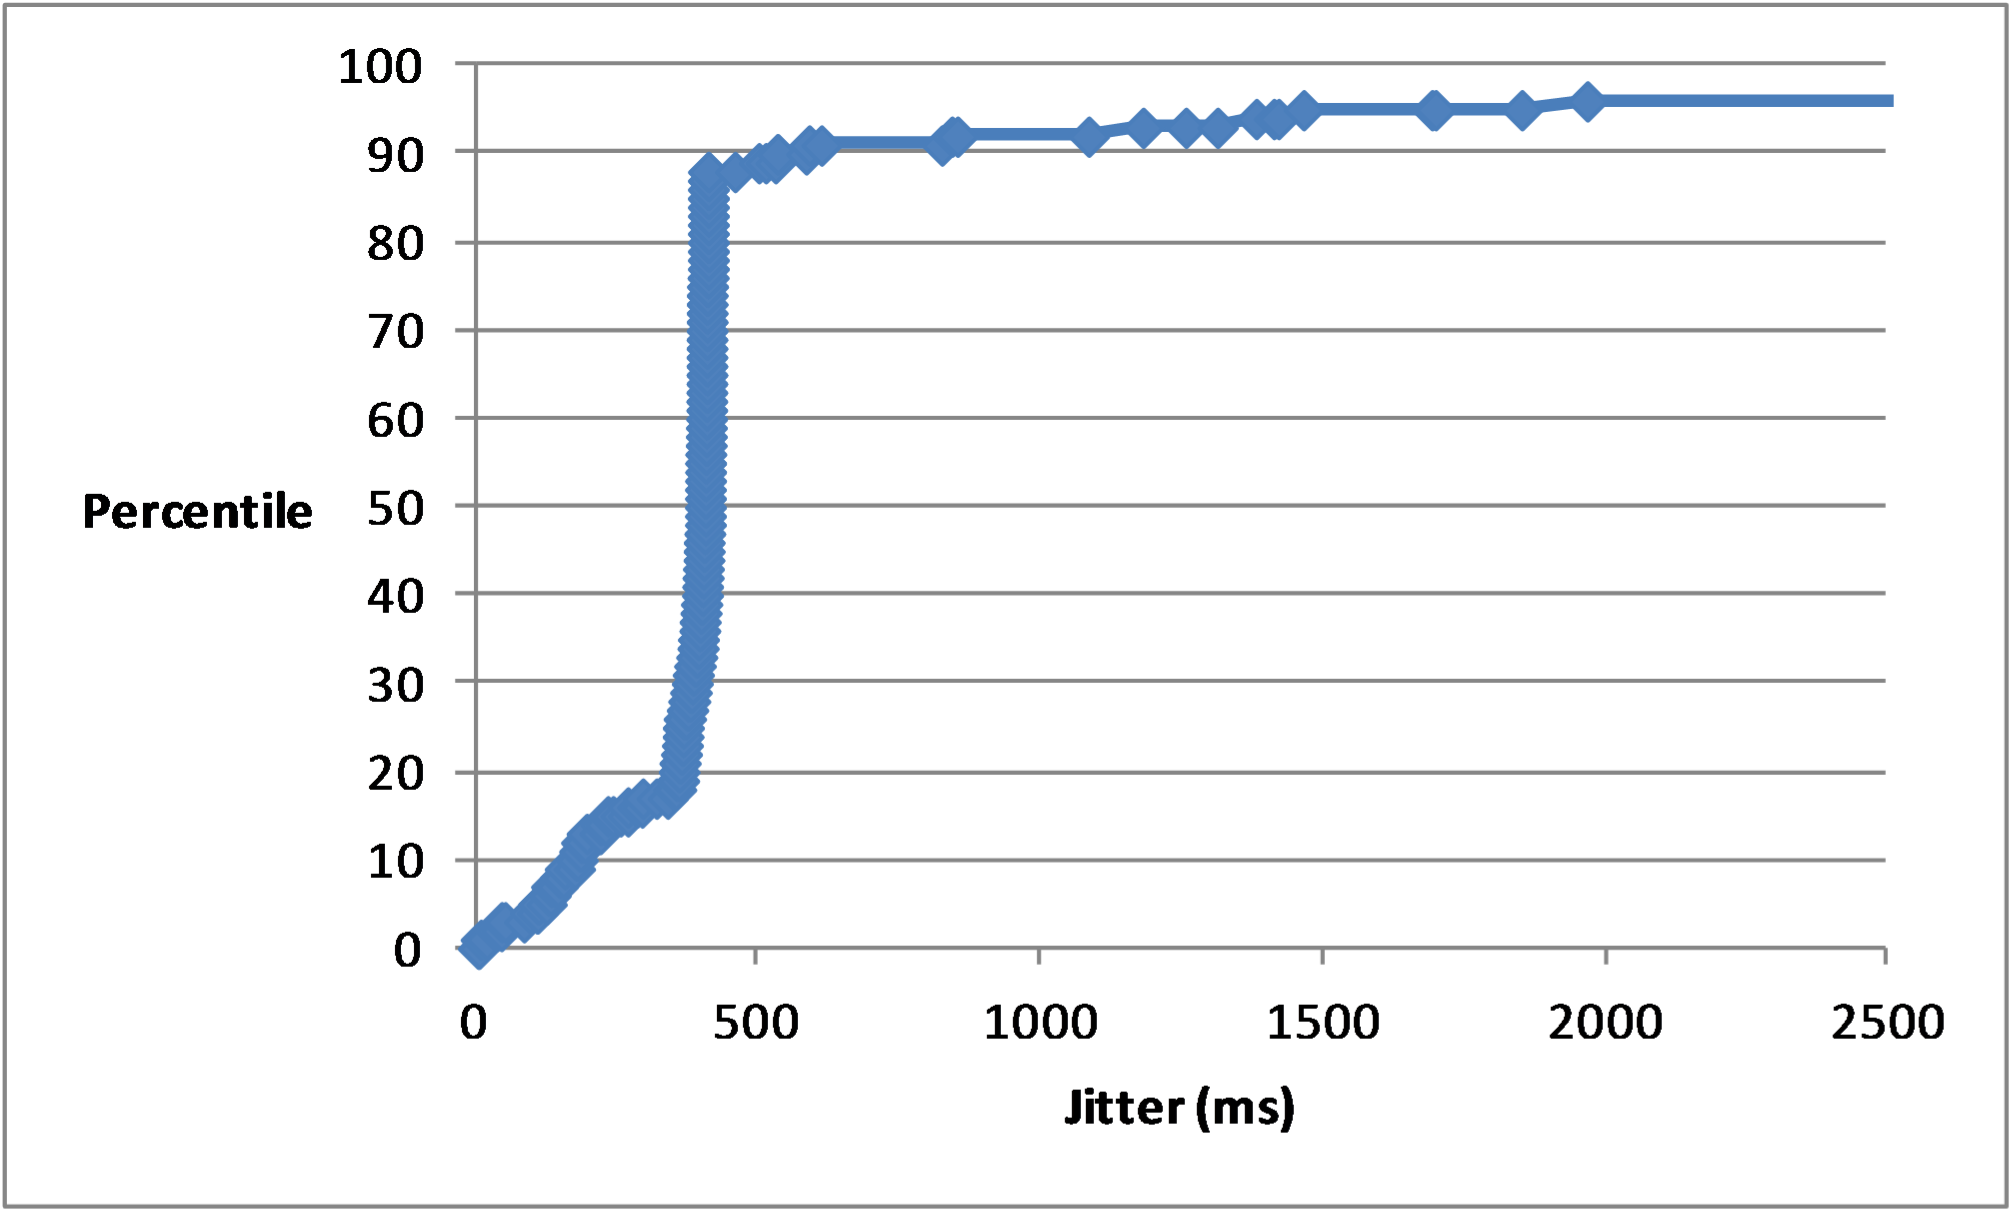
\includegraphics[width=0.45\textwidth]{pics/dccp_10_jitter_closeup}}
   \subfloat[TCP.]{
      \label{fig:tcp_10_jitter_closeup}
      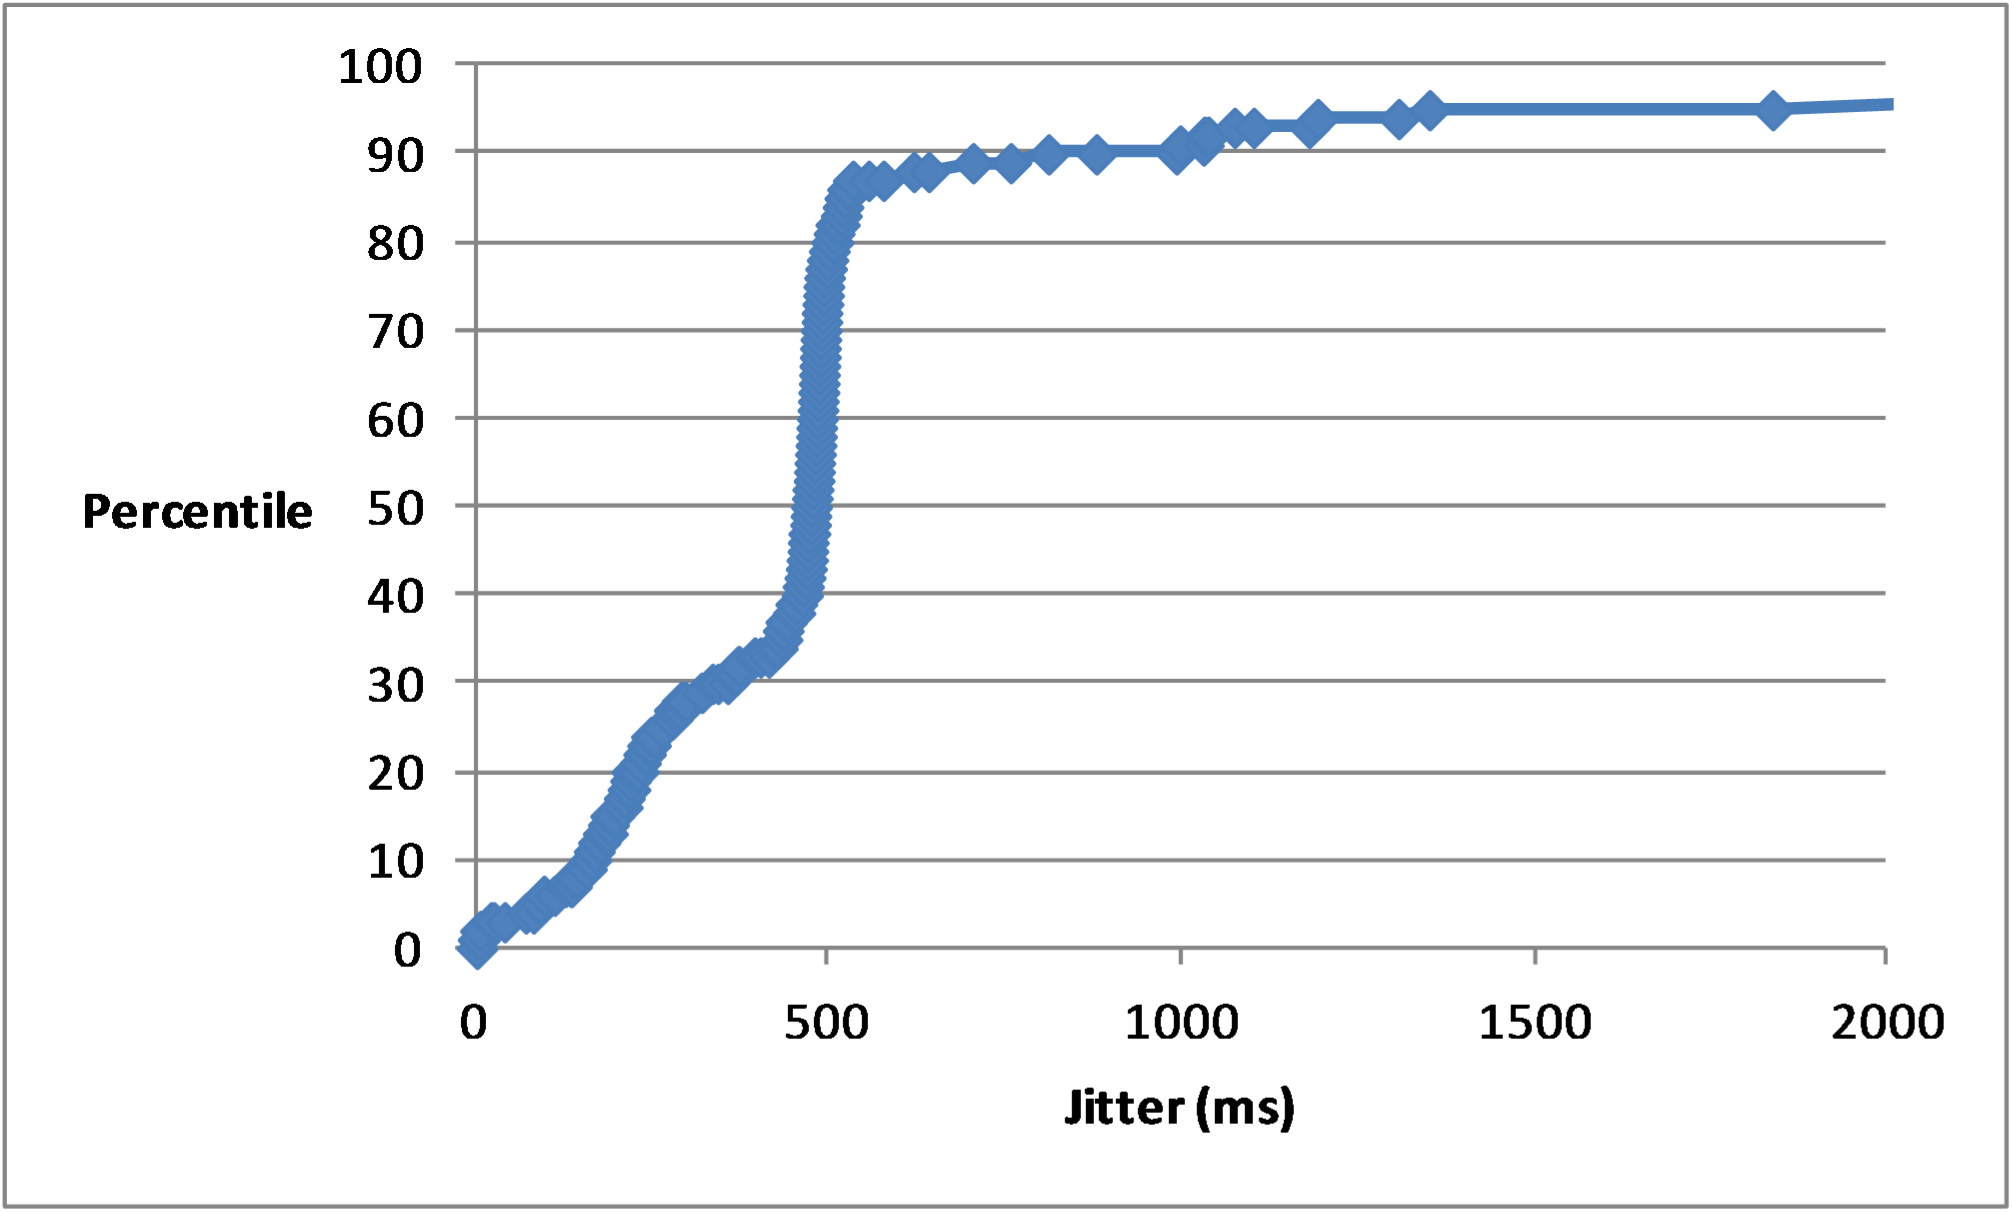
\includegraphics[width=0.45\textwidth]{pics/tcp_10_jitter_closeup}}
  \\ \subfloat[UDP.]{
      \label{fig:udp_10_jitter_closeup}
      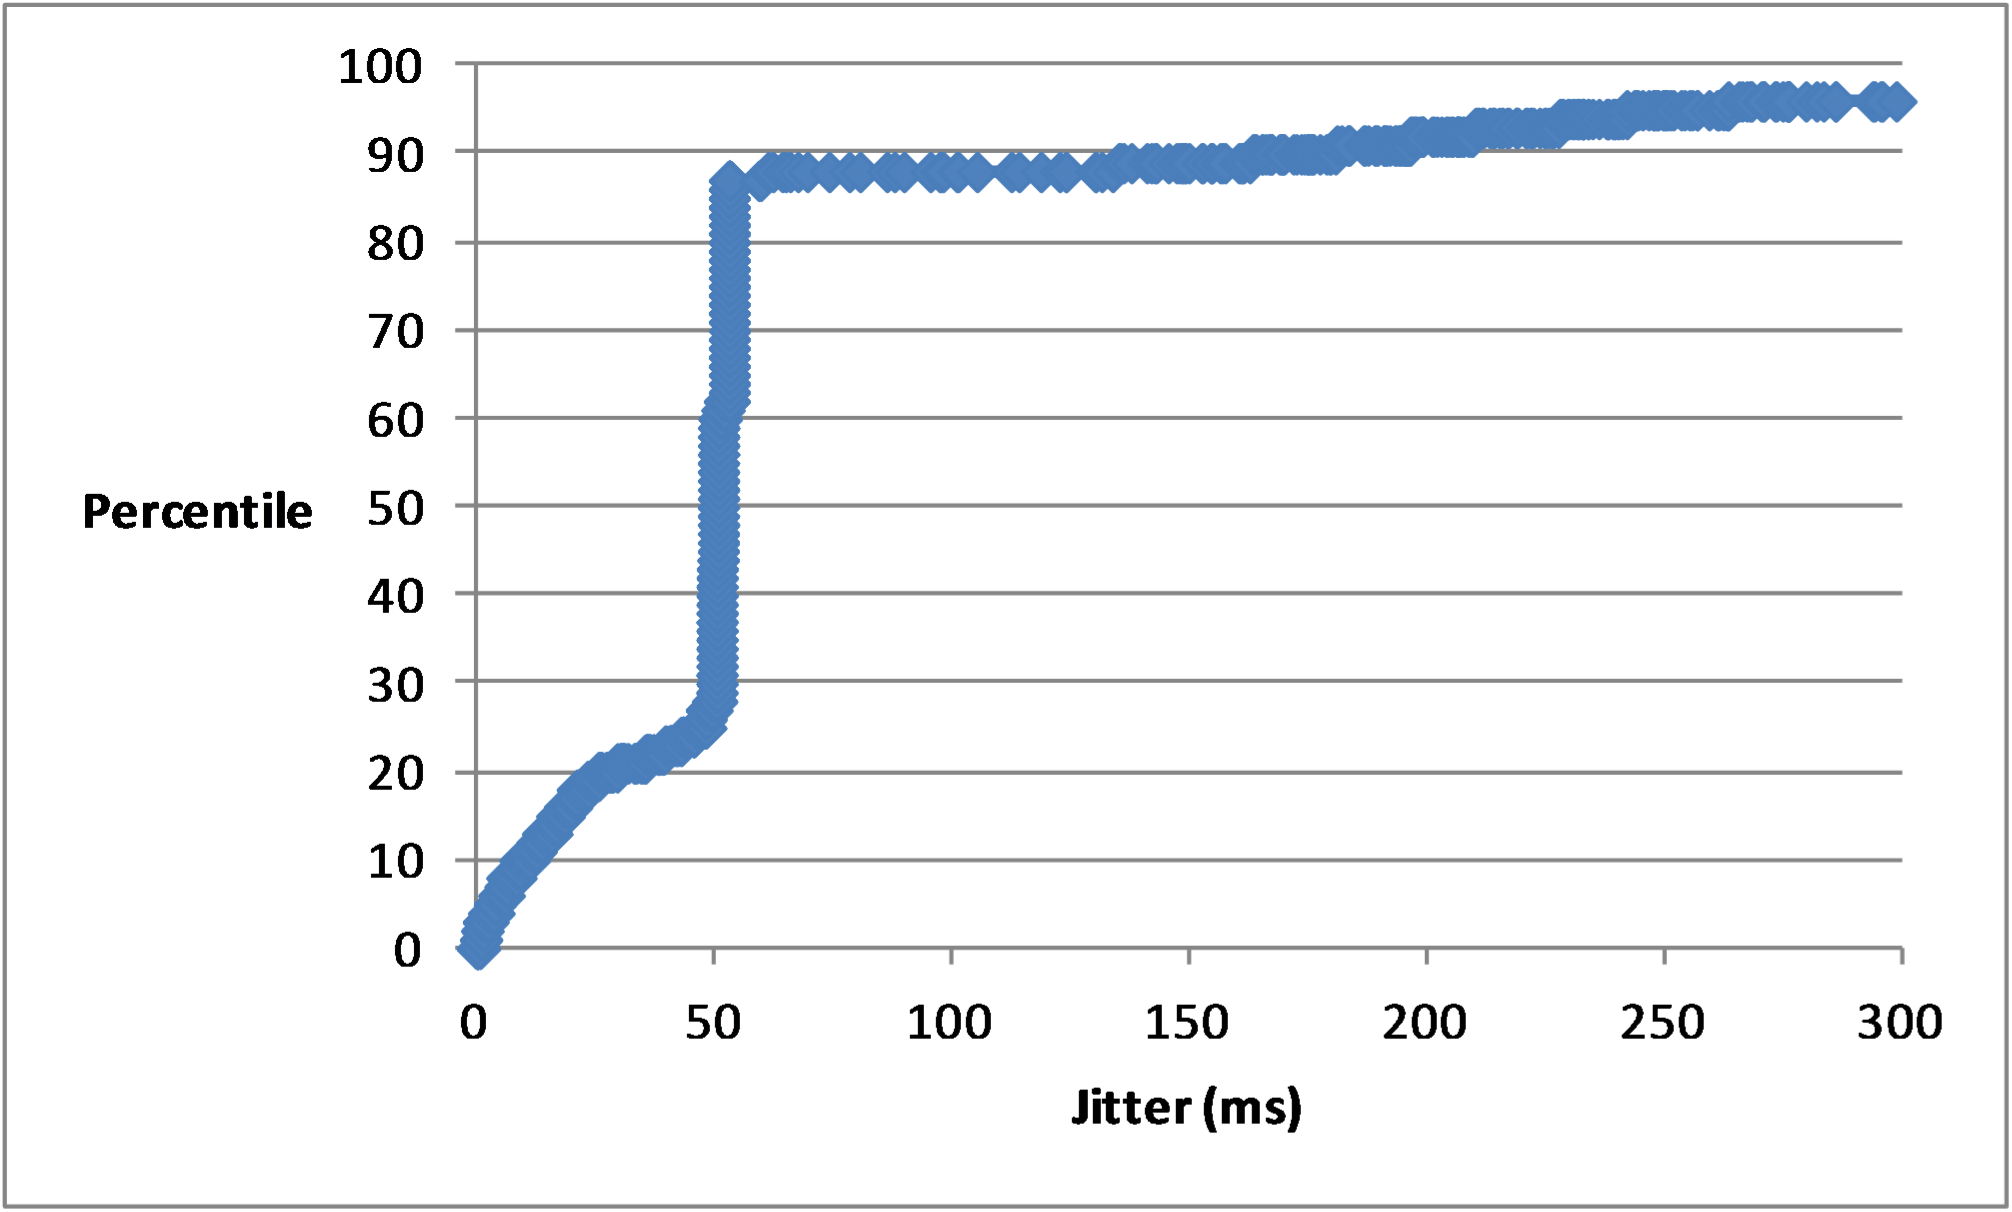
\includegraphics[width=0.45\textwidth]{pics/udp_10_jitter_closeup}}
   \caption{Detailed jitter CDFs for 10 Mbit/s.}
\label{fig:jitter_detail_10}
\end{figure*}

With no background traffic, all three protocols' jitter is concentrated at
approximately 5 ms, although TCP's jitter appears less uniform than that of DCCP
and UDP.

With 9 Mbit/s, differences begin to emerge. Approximately 90\% of DCCP's jitter
measurements are below 700 ms, with a significant majority of that 90\% lying
between roughly 600 ms and 700 ms. For TCP, about 90\% of its jitter values are
less than or equal to 500 ms, and roughly half of those measurements fall
between approximately 400 ms and 450 ms. In contrast, most of UDP's jitter
measurements at this level are at or below roughly 50 ms., and approximately
40\% fall between 40 ms and 50 ms.

At 10 Mbit/s, nearly 90\% of DCCP's jitter is less than about 400 ms, and
roughly 70\% is between approximately 300 ms and 400 ms. TCP's jitter is
concentrated primarily at or below 500 ms, with roughly 50\% falling between 400
ms and 500 ms. Finally, slightly over 90\% of UDP's jitter measurements are less
than 200 ms, with the majority of those values concentrated near 50 ms.

From this analysis, we can conclude that UDP is significantly less prone to
jitter than either DCCP or TCP during severe congestion. Since both DCCP and TCP
implement congestion control where UDP does not, it appears that congestion
control may drastically worsen jitter in such scenarios.



\section{Conclusion}
\label{sec:concl}

We found that UDP was the least affected by network congestion in terms of its sending rate, while DCCP was not significantly affected between 9Mbits/s and 10Mbits/s with regards to packet loss and jitter.  Between DCCP and TCP, DCCP had a higher average packet loss percentage than the other two protocols. DCCP also had a lower amount of jitter over the congested network, whereas TCP had a higher amount of jitter. Our results suggest that the congestion contol system implemented in DCCP behaves similar to TCP's congestion control, except with a slightly higher packet loss percentage. This was expected, since the authors of DCCP modeled their congestion control algorithm closely to TCP's congestion control. An unexpected result we did find was that DCCP didn't have as large of a difference in packet loss as TCP. This may be attributed to our small network setup (2 computers) as well as testing only on a local network.  When running over the internet, higher delays could occur with an increased likelihood of lost packets due to many environment variables introduced.  This should be a focus for future work.

\balance
\bibliography{references}
\end{document}
